\chapter{Forecasting the Disturbance Storm Time Index: Gaussian Process Models}\label{chapter:dst_osa}

{\small
    We present a methodology for generating probabilistic predictions for the 
    \emph{Disturbance Storm Time} ($\mathrm{Dst}$) geomagnetic activity index. We focus on the 
    \emph{One Step Ahead} (OSA) prediction task and use the OMNI hourly resolution data to build 
    our models. Our proposed methodology is based on the technique of 
    \emph{Gaussian Process Regression} (GPR). Within this framework we develop two models; 
    \emph{Gaussian Process Auto-Regressive} (GP-AR) and 
    \emph{Gaussian Process Auto-Regressive with eXogenous inputs} (GP-ARX). We also propose a 
    criterion to aid model selection with respect to the order of auto-regressive inputs. 
    Finally we test the performance of the GP-AR and GP-ARX models on a set of $63$ geomagnetic 
    storms between $1998$ and $2006$ and illustrate sample predictions with error bars for some of 
    these events.
}
        
\vfill
\sectionlinetwo{DarkGreen}{88}
\vfill

\noindent
    \parbox{\textwidth}{%
        {\small This chapter is based on the following:\\
        
        \textbf{Article}:\\
        \bibentry{ChandorkarDst}\\
        
        \textbf{Book Chapter}:\\
        \bibentry{CHANDORKAR2018237}}
    }%

\clearpage

\section{Introduction}


The magnetosphere's dynamics and its associated solar wind driver form a complex dynamical system. 
It is therefore instructive and greatly simplifying to use representative indices to quantify the 
state of geomagnetic activity.

Geomagnetic indices come in various forms, they may take continuous or discrete values and may be 
defined with varying time resolutions. Their values are often calculated by averaging or combining 
a number of readings taken by instruments, usually magnetometers, around the Earth. Each 
geomagnetic index is a proxy for a particular kind of phenomenon. Some popular indices are the 
$\mathrm{Kp}$, $\mathrm{Dst}$ and the $\mathrm{AE}$ index.


\begin{enumerate}
    \item $\mathrm{Kp}$: The Kp-index is a discrete valued global geomagnetic activity index and is 
    based on 3 hour measurements of the K-indices \citep{Bartels}. The K-index itself is a three 
    hour long quasi-logarithmic local index of the geomagnetic activity, relative to a calm day 
    curve for the given location.
    
    \item $\mathrm{AE}$: The Auroral Electrojet Index, $\mathrm{AE}$, is designed to provide a 
    global, quantitative measure of auroral zone magnetic activity produced by enhanced ionospheric 
    currents flowing below and within the auroral oval \citep{AEIndex}. It is a continuous index 
    which is calculated every hour.
    
    \item $\mathrm{Dst}$: A continuous hourly index which gives a measure of the weakening or 
    strengthening of the Earth's equatorial magnetic field due to particle injection in the 
    magnetosphere. Particle injection has a number of sources such as, weakening or strengthening 
    of the ring currents and the geomagnetic storms \citep{DesslerAndParker}, near Earth cross tail 
    current \citep{ganushkina2004long,angeo-28-123-2010}, partial ring current 
    \citep{JGRA:JGRA15878}, substorm current wedge \citep{JGRA:JGRA15211}, magnetopause current, 
    etc. 
\end{enumerate}

%Talk about Burton and friends
For the present study, we focus on prediction of the hourly $\mathrm{Dst}$ index which is a 
straightforward indicator of geomagnetic storms. More specifically, we focus on the 
\emph{one step ahead} (OSA) (in this case one hour ahead) prediction of $\mathrm{Dst}$ because it 
is the simplest model towards building long term predictions of geomagnetic response of the Earth 
to changing space weather conditions. 

The $\mathrm{Dst}$ OSA prediction problem has been the subject of several modeling efforts in the 
literature. One of the earliest models has been presented by \citet{JGR:JGR10260} who calculated 
$\mathrm{Dst}(t)$ as the solution of an \emph{Ordinary Differential Equation} (ODE) which expressed 
the rate of change of $\mathrm{Dst}(t)$ as a combination of two terms: decay and injection 
$\frac{d}{dt} \mathrm{Dst}(t) = Q(t) - \frac{\mathrm{Dst}(t)}{\tau}$, where $Q(t)$ relates to the 
particle injection from the plasma sheet into the inner magnetosphere. 

The \citet{JGR:JGR10260} model has proven to be very influential particularly due to its 
simplicity. Many subsequent works have modified the proposed ODE by proposing alternative 
expressions for the injection term $Q(t)$ \citep{Wang:Dst,JGRA:JGRA14856}. More recently 
\citet{Ballatore2014} have tried to generate empirical estimates for the injection and decay terms 
in Burton's equation.

%Talk about NARMAX Dst
Another important empirical model used to predict $\mathrm{Dst}$ is the 
\emph{Nonlinear Auto-Regressive Moving Average with eXogenous inputs} (NARMAX) methodology 
\citep{doi:10.1080/00207178908559767,GRL:GRL13494,GRL:GRL20944,JGRA:JGRA18657,balikhin:narmax,JGRA:JGRA20661,JGRA:JGRA50192}. The NARMAX methodology builds models by constructing polynomial expansions of 
inputs and determines the best combinations of monomials to include in the refined model by using a 
criterion called the \emph{error reduction ratio} (ERR). The parameters of the well known NARMAX 
OLS-ERR model are calculated by solving the \emph{ordinary least squares} (OLS) problem arising 
from a quadratic objective function. It must be noted that the NARMAX methodology is not limited to 
polynomial functions, rather any set of basis function expansions can be used with it, such as 
radial basis functions, wavelets etc \citep{doi:10.1080/00207720600903011,JGRA:JGRA17327}. The 
reader may refer to \citet{billings2013nonlinear} for a detailed exposition of the NARMAX 
methodology.

%Talk about neural networks
Yet another family of forecasting methods is based on \emph{Artificial Neural Networks} (ANN) that 
have been a popular choice for building predictive models. Researchers have employed both the 
standard \emph{feed forward} and the more specialised \emph{recurrent} architectures. \citet{Lund} 
proposed an \emph{Elman} recurrent network architecture called Lund $\mathrm{Dst}$, which used the 
solar wind velocity, \emph{interplanetary magnetic field} (IMF) and historical $\mathrm{Dst}$ data 
as inputs. \citet{JGRA:JGRA17461} used recurrent neural networks to predict $\mathrm{Kp}$. 
\citet{SWE:SWE286} originally proposed a \emph{feed forward} network for predicting the 
$\mathrm{Kp}$ index which used the \emph{Boyle coupling function} \citet{boyle1997empirical}. The 
same architecture is adapted for prediction of $\mathrm{Dst}$ in \citet{SWE:SWE286}, popularly 
known as the Rice $\mathrm{Dst}$ model. \citet{pallocchia:hal-00318011} proposed a 
\emph{neural network} model called EDDA to predict $\mathrm{Dst}$ using only the IMF data.

%Local neurofuzzy modelling and singular spectrum analysis.
Apart from the NARMAX and neural network approaches, fuzzy methods have also been applied for 
$\mathrm{Dst}$ prediction, \citet{SWE:SWE146,Sharifi2006} outline the application of 
\emph{local neurofuzzy} models for one hour and two hour predictions of $\mathrm{Dst}$ 
respectively. Local neurofuzzy models reduce the input space into a number of regions each with its 
own expert predictor. The combined model predicts $\mathrm{Dst}$ for a new point as a linear 
combinations of the predictions from each expert weighted by a fuzzy score signifying the 
importance of each model for the provided input. For improving predictive performance of two hour 
$\mathrm{Dst}$ forecasts in \citet{Sharifi2006}, the authors use \emph{singular spectrum analysis} 
(SSA). Singular spectrum analysis consists of extracting orthogonal components from a lagged time 
series, it is equivalent to \emph{principal component analysis} (PCA) which is quite extensively 
used in the machine learning community. \citet{loskutov2001testing,loskutov2001study} provide a 
good background to the theory and application of SSA to geomagnetic time series.

%Talk about need for probabilistic forecasts.
Although much research has been done on prediction of the $\mathrm{Dst}$ index, much less has been 
done on probabilistic forecasting of $\mathrm{Dst}$. One such work described in 
\citet{McPherron:2013} involves identification of high speed solar wind streams using the WSA model 
\citep{WSAModel}, using predictions of high speed streams to construct ensembles of $\mathrm{Dst}$ 
trajectories which yield the quartiles of $\mathrm{Dst}$ time series. 

A simple way to construct error bars on the predictions of forecasting models is by using the well 
known \textit{past cast} performance i.e. by calculating the standard deviations of the predictions 
generated by the model on a hold out data set. One limitation of such an approach is that the 
variance of the model predictions is computed once and for all. It does not adapt according to the 
inputs provided to the model. This may lead to overestimation or underestimation of the uncertainty 
around a given prediction, depending on the prevalent geo-magnetic conditions and the data set used 
to calculate the \textit{past cast} model performance.

In this work we propose a technique for probabilistic forecasting of $\mathrm{Dst}$, which yields a 
predictive distribution as a closed form expression. Our models take as input past values of 
$\mathrm{Dst}$, solar wind speed and the \textit{z} component of the 
\emph{Interplanetary Magnetic Field} (IMF) and output a Gaussian distribution with a specific mean 
and variance as the OSA prediction of the $\mathrm{Dst}$. 

We use the \emph{Gaussian Process Regression} methodology to construct auto-regressive models for 
$\mathrm{Dst}$ and show how to perform exact inference in this framework. We further outline a 
methodology to perform model selection with respect to its free parameters and time histories.

The remainder of this chapter is organised as follows: Section \S~\ref{sec:osaGPmethod} gives the 
reader an overview of the history of \emph{Gaussian Process} models as well as how they are 
formulated and how to perform inference with them. Sections \S~\ref{sec:osa}, \S~\ref{sec:gpar}, 
\S~\ref{sec:gparx} \& \S~\ref{sec:modeltraining} describe the GP-AR and GP-ARX models for OSA 
prediction of $\mathrm{Dst}$ and how to choose their free parameters for better performance. 
Sections \S~\ref{sec:gpOSAEval} \& \S~\ref{sec:res} evaluate the performance of the proposed 
GP-AR and GP-ARX models.

\section{Methodology: Gaussian Process} \label{sec:osaGPmethod}

\emph{Gaussian Processes} first appeared in machine learning research in 
\citet{Neal:1996:BLN:525544}, as the limiting case of Bayesian inference performed on neural 
networks with infinitely many neurons in the hidden layers. Although their inception in the machine 
learning community is recent, their origins can be traced back to the geo-statistics research 
community where they are known as \emph{Kriging} methods \citep{krige1951statistical}. In pure 
mathematics area \emph{Gaussian Processes} have been studied extensively and their existence was 
first proven by Kolmogorov's extension theorem \citep{tao2011introduction}. The reader is referred 
to \citet{Rasmussen:2005:GPM:1162254} for an in-depth treatment of Gaussian Processes in 
machine learning.

Let us assume that we want to model a process in which a scalar quantity $y$ is specified as 
$y = f(\mathbf{x}) + \epsilon$ where   $f(.): \mathbb{R}^d \rightarrow \mathbb{R}$ is an unknown 
scalar function of a multidimensional input vector $\mathbf{x} \in \mathbb{R}^d$, $d$ is the 
dimensionality of the input space, and $\epsilon \sim \mathcal{N}(0, \sigma^2)$ is zero mean 
Gaussian noise with variance $\sigma^2$.

A set of labeled data points ${(\mathbf{x}_i, y_i); i = 1 \cdots N}$ can be conveniently expressed 
by a $N \times d$ data matrix $\mathbf{X}$ and a $N \times 1$ response vector $\mathbf{y}$, as 
shown in \cref{eq:feat,eq:labels}.
%
\begin{align}
  \mathbf{X}  = & \left( \begin{array}{c} \mathbf{x}^{T}_1 \\ \mathbf{x}^{T}_2 \\ \vdots \\ \mathbf{x}^{T}_N \end{array} \right)_{N \times d} \label{eq:feat} \\
  \vspace{2\baselineskip}
  \mathbf{y}  = & \left( \begin{array}{c} y_1 \\ y_2 \\ \vdots \\ y_N \end{array} \right) _{N \times 1} \label{eq:labels}
\end{align}
%
Our task is to infer the values of the unknown function $f(.)$ based on the inputs $\mathbf{X}$ and 
the noisy observations $\mathbf{y}$. We now assume that the joint distribution of 
$f(\mathbf{x}_i), i = 1 \cdots N$ is a multivariate Gaussian as shown in 
\cref{eq:fvalues,eq:normal,eq:sto}.
%
\begin{align}
 \mathbf{f} = & \left( \begin{array}{c} f(\mathbf{x}_1) \\ f(\mathbf{x}_2) \\ \vdots \\ f(\mathbf{x}_N) \end{array} \right) \label{eq:fvalues}\\
 \vspace{2\baselineskip}
 \mathbf{f} | \mathbf{x}_1, \cdots, \mathbf{x}_N \sim & \mathcal{N}\left( \mathbf{\mu}, \mathbf{\Lambda} \right)  \label{eq:normal}\\
 \vspace{2\baselineskip}
 p( \mathbf{f} \ | \ \mathbf{x}_1, \cdots, \mathbf{x}_N) = & \frac{1}{(2\pi)^{n/2} \det(\mathbf{\Lambda})^{1/2}} \exp \left(-\frac{1}{2} (\mathbf{f} - \mathbf{\mu})^T \mathbf{\Lambda}^{-1} (\mathbf{f} - \mathbf{\mu}) \right) \label{eq:sto}
\end{align}
%
Here $\mathbf{f}$ is a $N\times 1$ vector consisting of the values 
$f(\mathbf{x}_i), i = 1 \cdots N$. In \cref{eq:normal}, 
$\mathbf{f}|\mathbf{x}_1, \cdots, \mathbf{x}_N$ denotes the conditional distribution of 
$\mathbf{f}$ with respect to the input data (i.e., $\mathbf{X}$) and 
$\mathcal{N}\left(\mathbf{\mu}, \mathbf{\Lambda} \right)$ represents a multivariate Gaussian 
distribution with mean vector $\mathbf{\mu}$ and covariance matrix $\mathbf{\Lambda}$. The 
probability density function of this distribution 
$p( \mathbf{f} \ | \ \mathbf{x}_1, \cdots, \mathbf{x}_N)$ is therefore given by \cref{eq:sto}.

From \cref{eq:sto}, one can observe that in order to uniquely define the distribution of the 
process, it is required to specify $\mathbf{\mu}$ and $\mathbf{\Lambda}$. For this probability 
density to be valid, there are further requirements imposed on $\mathbf{\Lambda}$: 


\begin{enumerate}
      \item Symmetry: 
            $\mathbf{\Lambda}_{ij} = \mathbf{\Lambda}_{ji} \ \forall i,j \in {1, \cdots, N} $ 
      \item Positive Semi-definiteness: 
            $\mathbf{z}^T \mathbf{\Lambda} \mathbf{z} \geq 0 \ \forall \mathbf{z} \in \mathbb{R}^N$  
\end{enumerate}

Inspecting the individual elements of $\mathbf{\mu}$ and $\mathbf{\Lambda}$, we realise that they 
take the following form.
%
\begin{align}
      \mu_i = & \mathbb{E}[f(\mathbf{x}_i)] := m(\mathbf{x}_i) \\
      \Lambda_{ij} = & \mathbb{E}[(f(\mathbf{x}_i) - \mu_i)(f(\mathbf{x}_j) - \mu_j)] := K(\mathbf{x}_i, \mathbf{x}_j)
\end{align}
%
Here $\mathbb{E}$ denotes the expectation (average). The elements of $\mathbf{\mu}$ and 
$\mathbf{\Lambda}$ are expressed as functions $m(\mathbf{x}_i)$ and $K(\mathbf{x}_i, \mathbf{x}_j)$ 
of the inputs $\mathbf{x}_i,\ \mathbf{x}_j$. Specifying the functions $m(\mathbf{x})$ and 
$K(\mathbf{x}, \mathbf{x}')$ completely specifies each element of 
$\mathbf{\mu}$ and $\mathbf{\Lambda}$ and subsequently the finite dimensional distribution of 
$\mathbf{f} | \mathbf{x}_1, \cdots, \mathbf{x}_N $. In most practical applications of 
\emph{Gaussian Processes} the mean function is often defined as $m(\mathbf{x}) = 0$, which is not 
unreasonable if the data is standardised to have zero mean. \emph{Gaussian Processes} are 
represented in machine learning literature using the following notation:
%
\begin{equation}\label{eq:gpformulation}
    f(\mathbf{x}) \sim \mathcal{GP}(m(\mathbf{x}), K(\mathbf{x}, \mathbf{x}'))
\end{equation}

\subsection{Inference and Predictions} \label{sec:inference}

Our aim is to infer the function $f(\mathbf{x})$ from the noisy training data and generate 
predictions $f(\mathbf{x}^{*}_i)$ for a set of test points 
${\mathbf{x}^{*}_i : \forall i \in 1, \cdots, M}$. We define $\mathbf{X}^*$ as the test data 
matrix whose rows are formed by $\mathbf{x}^{*}_i$ as shown in \cref{eq:testfeat}. 
%
\begin{equation}
    \mathbf{X}_* = \left( \begin{array}{c} (\mathbf{x}^{*}_1)^T \\ (\mathbf{x}^{*}_2)^T \\ \vdots \\ (\mathbf{x}^{*}_M)^T \end{array} \right)_{M \times d} \label{eq:testfeat} 
\end{equation}
%
Using the multivariate Gaussian distribution in \cref{eq:sto} we can construct the joint 
distribution of $f(\mathbf{x})$ over the training and test points. The vector of training and test 
outputs $\left( \begin{array}{c} \mathbf{y} \\ \mathbf{f_*} \end{array} \right)$ is of dimension 
$(N+M) \times 1$ and is constructed by appending the test set predictions $\mathbf{f}_*$ to the 
observed noisy measurements $\mathbf{y}$.
%
\begin{align}
    \mathbf{f}_* = & \left( \begin{array}{c} f(\mathbf{x^{*}_1}) \\ f(\mathbf{x^{*}_2}) \\ \vdots \\ f(\mathbf{x^{*}_M}) \end{array} \right)_{M \times 1} \\
     \vspace{4\baselineskip}
    \left( \begin{array}{c} \mathbf{y} \\ \mathbf{f_*} \end{array} \right) | \ \ \mathbf{X}, \mathbf{X}_* \sim & 
    \mathcal{N}\left(\mathbf{0}, \left[ \begin{array}{cc} \mathbf{K} + \sigma^{2} \mathbf{I} & \mathbf{K}_{*} \\ \mathbf{K}_{*}^T & \mathbf{K}_{**} \end{array} \right ] \right) \label{eq:dist}
\end{align}
%
Since we have noisy measurements of $f$ over the training data, we add the noise variance 
$\sigma^2$ to the variance of $f$ as shown in \cref{eq:dist}. The block matrix components of the 
$(N+M) \times (N+M)$ covariance matrix have the following structure.

\begin{enumerate}
      \item $\mathbf{I}$: The $N \times N$ identity matrix.
      \item $\mathbf{K} = [K(\mathbf{x}_i, \mathbf{x}_j)], \ i,j \in 1,\cdots,N$: 
            Kernel matrix constructed from all couples obtained from the training data.
      \item $\mathbf{K}_{*} = [K(\mathbf{x}_i, \mathbf{x}^{*}_j)], \ i \in 1,\cdots,N ; j \in 1,\cdots,M$: 
            Cross kernel matrix constructed from all couples between training and test data points.
      \item $\mathbf{K}_{**} = [K(\mathbf{x}^{*}_i, \mathbf{x}^{*}_j)], \ i,j \in 1,\cdots,M$: 
            Kernel matrix constructed from all couples obtained from the test data.
\end{enumerate}

With the multivariate normal distribution defined in \cref{eq:dist}, probabilistic predictions 
$f_*$ can be generated by constructing the conditional distribution 
$\mathbf{f_*}|\mathbf{X},\mathbf{y},\mathbf{X_*}$. Since the original distribution of 
$\left( \begin{array}{c} \mathbf{y} \\ \mathbf{f_*} \end{array} \right) | \ \ \mathbf{X}, \mathbf{X}_*$ 
is a multivariate Gaussian, conditioning on a subset of elements $\mathbf{y}$ yields another 
Gaussian distribution whose mean and covariance can be calculated exactly, as in 
\cref{eq:posterior} \citep{Rasmussen:2005:GPM:1162254}.
%
\begin{equation}
    \mathbf{f_*}|\mathbf{X},\mathbf{y},\mathbf{X_*} \sim \mathcal{N}(\mathbf{\bar{f}_*}, \Sigma_*)  \label{eq:posterior},
\end{equation}
where
\begin{align}
    \mathbf{\bar{f}_*} = & \mathbf{K}^T_{*} [\mathbf{K} + \sigma^{2} \mathbf{I}]^{-1} \mathbf{y} \label{eq:posteriormean} \\
    \Sigma_* = & \mathbf{K}_{**} - \mathbf{K}^T_{*} \left(\mathbf{K} + \sigma^{2} \mathbf{I}\right)^{-1} \mathbf{K}_{*} \label{eq:posteriorcov}
\end{align}

The practical implementation of \emph{Gaussian Process} models requires the inversion of the 
training data kernel matrix $[\mathbf{K} + \sigma^{2} \mathbf{I}]^{-1}$ to calculate the parameters 
of the predictive distribution $\mathbf{f_*}|\mathbf{X},\mathbf{y},\mathbf{X_*}$. The computational 
complexity of this inference is dominated by the linear problem in \cref{eq:posteriormean}, which 
can be solved via Cholesky decomposition, with a time complexity of $O(N^3)$, where $N$ is the 
number of data points.

The distribution of $\mathbf{f_*}| \mathbf{X},\mathbf{y},\mathbf{X_*}$ is known in Bayesian 
analysis as the \emph{Posterior Predictive Distribution}. This illustrates a key difference between 
\emph{Gaussian Processes} and other regression models such as \emph{Neural Networks}, 
\emph{Linear Models} and \emph{Support Vector Machines}: a \emph{Gaussian Process} model does not 
generate point predictions for new data but outputs a predictive distribution for the quantity 
sought, thus allowing to construct error bars on the predictions. This property of Bayesian models 
such as \emph{Gaussian Processes} makes them very appealing for Space Weather forecasting 
applications. 

The central design issue in applying \emph{Gaussian Process} models is the choice of the function 
$K(\mathbf{x}, \mathbf{x}')$. The same constraints that apply to $\mathbf{\Lambda}$ also apply to 
the function $K$. In machine learning, these symmetric positive definite functions of two variables 
are known as covariance functions or \emph{kernels}. Kernel based methods are applied extensively 
in data analysis \citep{Scholkopf:2001:LKS:559923,hofmann2008} i.e. regression, clustering, 
classification, density estimation \citep{Girolami:2002:OSD:638929.638938}.

\begin{table}[ht]
    \caption{Popular Kernel functions used in GPR models}
    \centering
    \begin{tabular}{l l l}
    \hline
     \textbf{Name}  & \textbf{Expression} & \textbf{Hyperparameters}  \\
    \hline
      {\small Radial Basis Function (RBF)}  & ${\scriptstyle \frac{1}{2} \exp(-||\mathbf{x} - \mathbf{y}||^2/l^2)}$  & ${\scriptstyle l \in \mathbb{R}}$   \\
      
      {\small Polynomial}  & ${\scriptstyle (\mathbf{x}\boldsymbol{\cdot} \mathbf{y} + b)^d}$ & ${\scriptstyle b \in \mathbb{R}, d \in \mathbb{N}}$   \\
      
      {\small Laplacian}  & ${\scriptstyle \exp(-||\mathbf{x} - \mathbf{y}||_{1}/\theta)}$  & ${\scriptstyle \theta \in \mathbb{R}^+}$  \\
      
      {\small Student's T}  & ${\scriptstyle 1/(1 + ||\mathbf{x} - \mathbf{y}||_{2}^d)}$ & ${\scriptstyle d \in \mathbb{R}^{+}}$\\
      
      {\small Maximum Likelihood Perceptron (MLP)}  & ${\scriptstyle \sin^{-1}\left(\frac{w\mathbf{x}\boldsymbol{\cdot} \mathbf{y} + b}{\sqrt{w\mathbf{x}\boldsymbol{\cdot} \mathbf{x} + b + 1} \sqrt{w\mathbf{y}\boldsymbol{\cdot} \mathbf{y} + b + 1}}\right)}$ & ${\scriptstyle w, b \in \mathbb{R}^{+}}$\\
    \hline
    \end{tabular}
    \label{table:kernel}
\end{table}
    
\subsection{Kernel Functions}

For the success of a \emph{Gaussian Process} model an appropriate choice of kernel function is 
paramount. The symmetry and positive semi-definiteness of \emph{Gaussian Process} kernels implies 
that they represent inner-products between some basis function representation of the data. The 
interested reader is suggested to refer to 
\citet{Berlinet2004,Scholkopf:2001:LKS:559923,hofmann2008} for a thorough treatment of kernel 
functions and the rich theory behind them. Some common kernel functions used in machine learning 
are listed in \cref{table:kernel}. 

The quantities $l$ in the RBF, and $b$ and $d$ in the polynomial kernel are known as 
\emph{hyper-parameters}. Hyper-parameters give flexibility to a particular kernel structure, for 
example $d = 1, 2, 3, \cdots$ in the polynomial kernel represents linear, quadratic, cubic and 
higher order polynomials respectively. The process of assigning values to the 
\emph{hyper-parameters} is crucial in the model building process and is known as 
\emph{model selection}. 

\subsection{Model Selection}\label{sec:gpModelSelection}

Given a GP model with a kernel function $K_\theta$, the problem of model selection consists of 
finding appropriate values for the kernel hyper-parameters 
$\theta = \left(\theta_1, \theta_2, \cdots, \theta_i\right)$. In order to assign a value to 
$\theta$, we must define an objective function which represents our confidence that the GP model 
built from a particular value of $\theta$ is the best performing model. Since GP models encode 
assumptions about the probability distribution of the output data $\mathbf{y}$ given inputs 
$\mathbf{X}$, it is natural to use the negative log-likelihood of the training data as a model 
selection criterion. 
%
\begin{align*}
  Q(\theta) & = - \text{log}(p(\mathbf{y}|\mathbf{X}, K_\theta)) \\
            & = -\frac{1}{2} \mathbf{y}\boldsymbol{\cdot} (\mathbf{K}_\theta + \sigma^{2} \mathbf{I})^{-1} \mathbf{y} - \frac{1}{2}|\mathbf{K}_\theta + \sigma^{2} \mathbf{I}| - \frac{N}{2}\text{log}(2\pi) \\
  \mathbf{K}_\theta & = [K_{\theta}(\mathbf{x}_i, \mathbf{x}_j)]_{N \times N}
\end{align*}
%
The model selection problem can now be expressed as the minimization problem shown below.
%
\begin{align*}
\theta^* = arg\min_{\theta} \ Q(\theta)
\end{align*}

The objective function $Q(\theta)$ in the general case can have multiple local minima, and 
evaluating the value of $Q(.)$ at any given $\theta$ requires inversion of the matrix 
$\mathbf{K}_\theta + \sigma^{2} \mathbf{I}$ which has a time complexity $O(N^3)$ as noted above. 
In the interest of saving computational cost, one cannot use exhaustive search through the domain 
of the hyper-parameters to inform our choice for $\theta$. Some of the techniques used for model 
selection in the context of GPR include.

\begin{enumerate}
\item Grid Search: Construct a grid of values for $\theta$ as the cartesian product of one 
      dimensional grids for each $\theta_i$, evaluate $Q(.)$ at each such grid point and choose the 
      configuration which yields minimum value of $Q(.)$.

\item Coupled Simulated Annealing: Introduced in \citet{Xavier-De-Souza2010}, it follows the same 
      procedure as \emph{grid search}, but after evaluation of the objective $Q(.)$ on the grid, 
      each grid point is iteratively mutated in a random walk fashion. This mutation is accepted or 
      rejected according to the new value of $Q(.)$ as well as its value on the other grid points. 
      This procedure is iterated until some stop criterion is reached.

\item Maximum Likelihood: This technique as outlined in \citet{Rasmussen:2005:GPM:1162254} is a 
      form of \emph{gradient descent}. It involves starting with an initial guess for $\theta$ and 
      iteratively improving it by calculating the gradient of $Q(.)$ with respect to $\theta$. 
      Although this method seems intuitive, it introduces an extra computational cost of 
      calculating the gradient of $Q(\theta)$ with respect to each $\theta_i$ in every iteration 
      and applying this method can sometimes lead to overfitting of the GPR model to the training 
      data \citet{Rasmussen:2005:GPM:1162254}.
\end{enumerate}

\section{One Step Ahead Prediction} \label{sec:osa}

Below in \cref{eq:Dst,eq:GPNoise,eq:DstGP} we outline a \emph{Gaussian Process} formulation for \emph{OSA} prediction of $ \mathrm{Dst}$. A vector of features $\mathbf{x}_{t-1}$ is used as input to an unknown function $f(\mathbf{x}_{t-1})$.

The features $ \mathbf{x}_{t-1}$ can be any collection of quantities in the hourly resolution OMNI data set. Generally $\mathbf{x}_{t-1}$ are time histories of $\mathrm{Dst}$ and other important variables such as plasma pressure $p(t)$, solar wind speed $V(t)$, $z$ component of the interplanetary magnetic field $B_z(t)$.
%
\begin{align}
    \mathrm{Dst}(t) & =  f(\mathbf{x}_{t-1}) + \epsilon \label{eq:Dst} \\
    \epsilon & \sim  \mathcal{N}(0, \sigma^2) \label{eq:GPNoise} \\
    f(x_t) & \sim  \mathcal{GP}(m(\mathbf{x}_t), K_{\text{osa}}(\mathbf{x}_t, \mathbf{x}_s)) \label{eq:DstGP}
\end{align}
%
We consider two choices for the input features $ \mathbf{x}_{t-1}$ leading to two variants of \emph{Gaussian Process} regression for $\mathrm{Dst}$ time series prediction.

\subsection{Gaussian Process Auto-Regressive (GP-AR)} \label{sec:gpar}

The simplest auto-regressive models for \emph{OSA} prediction of $\mathrm{Dst}$ are those that use only the history of $\mathrm{Dst}$ to construct input features for model training. The input features $\mathbf{x}_{t-1}$ at each time step are the history of $\mathrm{Dst}(t)$ until a time lag of $p$ hours.
%
\begin{equation}\label{eq:gpOSAAR}
    \mathbf{x}_{t-1} = \left(\mathrm{Dst}(t-1), \cdots , \mathrm{Dst}(t-p+1)\right)
\end{equation}
%
This description of the GP-AR model in \cref{eq:Dst,eq:GPNoise,eq:DstGP,eq:gpOSAAR}, as a Gaussian process $Dst(t)$ 
whose input space $\mathbf{x}(t)$ comprises previous realizations of itself has been discussed in time series 
\citep{roberts2013gaussian}, control systems \citep{kocijan2015modelling} and machine learning literature 
\citep{wang2006gaussian,wang2007gaussian}. The reader refer to appendix \ref{app:gpNARX} for detailed notes 
regarding GP time series models, some nuances of the GP-AR formulation and its relationship to auto-regressive 
time series models. 

\subsection{Gaussian Process Auto-Regressive with eXogenous inputs (GP-ARX)} \label{sec:gparx}

Auto-regressive models can be augmented by including exogenous quantities in the inputs $ \mathbf{x}_{t-1}$ at each time step, in order to improve predictive accuracy. While modeling $\mathrm{Dst}$ using the OMNI data, one must choose which solar wind quantities to include in the exogenous inputs of the predictive model. This choice is not straight forward and eventually requires a compromise between including important solar wind quantities and keeping the input space manageable in the interest of simplicity.

\subsubsection{Choice of Solar Wind Inputs}

$ \mathrm{Dst}$ gives a measure of ring currents, which are modulated by plasma sheet particle injections into the inner magnetosphere during sub-storms. Studies have shown that the substorm occurrence rate increases with solar wind velocity (high speed streams) \citet{Kissinger2011,Newell2016}. Prolonged southward interplanetary magnetic field (IMF) $z$-component ($B_z$) is needed for sub-storms to occur \citep{McPherron1986}. An increase in the solar wind electric field, $V_{\text{sw}}B_z$, can increase the dawn-dusk electric field in the magnetotail, which in turn determines the amount of plasma sheet particle that move to the inner magnetosphere \citet{Friedel2001}. 

Apart from $V$ and $B_z$, other quantities which have been shown to correlate with geomagnetic activity are solar wind dynamic pressure $P$, clock angle $tan \theta = \frac{B_y}{B_z}$, Akasofu $\epsilon$ \citep{1986AkasofuE} and solar wind magnetosphere coupling functions \citep{JGRA:JGRA21451}. 

Although solar wind magnetospheric coupling functions have been shown to have correlation with geomagnetic indices, they are expressed in terms of $V$ and $B_z$, and hence we do not include them as explicit inputs to the model. \emph{Gaussian Process} models derive their strength from automatic feature construction achieved by the covariance functions (interested readers may refer to chapters 6 and 7  in \citet{Rasmussen:2005:GPM:1162254}). As long as coupling functions can be approximated in the \emph{eigenspace} of the covariance function we need not make them explicit in the input features. 

Therefore, our exogenous parameters consist of solar wind velocity $ V_{\text{sw}}$ and IMF $B_z$. In this model we choose distinct time lags $p$, $p_{v}$ and $p_{b}$ for $\mathrm{Dst}$, $V$ and $B_z$ respectively.
%
\begin{align*}
       \mathbf{x}_{t-1} & = (\mathrm{Dst}(t-1), \cdots , \mathrm{Dst}(t-p+1), \\
        & \ \ \ \ \  V_{\text{sw}}(t-1), \cdots, V_{\text{sw}}(t-p_{v}+1),\\
        & \ \ \ \ \  B_{z}(t-1), \cdots, B_{z}(t-p_{b}+1))
\end{align*}
%
It is an important question as to how unaccounted inputs such as solar wind dynamic pressure $P$ and clock angle $\theta$ affect the structure of the GP-ARX model. From a model selection perspective, these unaccounted inputs should lead to higher values of the noise covariance. In the specific case of solar wind dynamic pressure, it is calculated as a product of the plasma density and the solar wind speed making it highly correlated with the solar wind speed, as a result the GP-ARX model can infer a large portion of the information content from the solar wind speed itself. With respect to the clock angle, it must be noted that coupling functions such as Akasofu $\epsilon$ generally contain powers of $\sin \theta$ bounding the effect of clock angle to an absolute magnitude of $1$, hence we do not expect these unaccounted inputs to greatly improve the predictive capabilities of the GP-ARX model.

\subsection{Choice of Mean Function}

Mean functions in GPR models encode trends in the data, they are the baseline predictions the model falls back to in case the training and test data have little correlation as predicted by the kernel function. If there is no prior knowledge about the function to be approximated, \citet{Rasmussen:2005:GPM:1162254} state that it is perfectly reasonable to choose $ m(\mathbf{x} = 0)$ as the mean function, as long as the target values are normalised. In the case of the $\mathrm{Dst}$ time series, it is known that the so called \emph{persistence model} 
$\mathrm{\hat{D}st}(t) = \mathrm{Dst}(t-1)$ has high correlation with \emph{OSA} $\mathrm{Dst}$. Due to its simplicity, we choose the \emph{persistence model} as the prior mean function in our OSA Dst models. 

The \emph{persistence model} can be described as \emph{Markovian} prediction mechanism, when it is chosen as the prior mean of the GP-AR and GP-ARX model, it is indeed the case that the prior probability distribution of $ \mathrm{Dst}(t)$ is Gaussian with a strong \emph{Markovian} behavior $P(\mathrm{Dst}(t)|\mathbf{x}_t) \sim \mathcal{N}(\mathrm{Dst}(t-1), \sqrt{K_{\text{osa}}(\mathbf{x}_t, \mathbf{x}_t)})$, but the posterior predictive distribution of $\mathrm{Dst}(t)$ conditional on the model training data (given in \cref{eq:posteriormean}) is non-\emph{Markovian} due its dependence on the term denoted by $\mathbf{K}_{*}$ which contains kernel values computed between the test data and training data features. Thus the GP-AR and GP-ARX models when used conditional on training data are non-\emph{Markovian} predictive models.

\subsection{Choice of Kernel}

In this study, we construct Gaussian Process regression models with a combination of the \emph{maximum likelihood perceptron} kernel and \emph{student's T} kernel as shown in \cref{eq:usedKernel}. The \emph{maximum likelihood perceptron} kernel is the \emph{Gaussian Process} equivalent of a single hidden layer feed-forward neural network model as demonstrated in \citet{Neal:1996:BLN:525544}.

\begin{align}
    K_{\text{osa}}(\mathbf{x}, \mathbf{y}) & = K_{\text{mlp}}(\mathbf{x}, \mathbf{y}) + K_{\text{st}}(\mathbf{x}, \mathbf{y}) \label{eq:usedKernel} \\
    K_{\text{mlp}}(\mathbf{x}, \mathbf{y}) & = \sin^{-1}\left(\frac{w\mathbf{x}\boldsymbol{\cdot} \mathbf{y} + b}{\sqrt{w\mathbf{x}\boldsymbol{\cdot} \mathbf{x} + b + 1} \sqrt{w\mathbf{y}\boldsymbol{\cdot} \mathbf{y} + b + 1}}\right) \\
    K_{\text{st}}(\mathbf{x}, \mathbf{y}) & = \frac{1}{1 + ||\mathbf{x} - \mathbf{y}||_{2}^d}
\end{align}

\section{Experiments} \label{sec:modeltraining}

\begin{table}[ht]
    \centering
    \caption{Settings of model selection procedures}
    \begin{tabular}{l c c c}
    \hline
    \textbf{Procedure} & \textbf{Grid Size} & \textbf{Step} & \textbf{Max Iterations} \\
    \hline
    Grid Search & $10$ & $0.2$ & NA \\
    Coupled Simulated Annealing & $4$ & $0.2$ & $30$ \\
    Maximum likelihood & NA & $0.2$ & $150$\\
    \hline
    \end{tabular}
    \label{table:modelselection}
\end{table}

\subsection*{Training}

We selected OMNI data sections 00:00 January 3 2010 to 23:00 January 23 2010 and 20:00 August 5 2011 to 22:00 August 6 2011 for training the GP-AR and GP-ARX models. The first training data section consists of ambient fluctuations of $ \mathrm{Dst}$ while the second contains a geomagnetic storm.

The computational complexity of calculation of the predictive distribution is $O(N^3)$, as discussed in section \S~\ref{sec:inference}. This can limit the size of the covariance matrix constructed from the training data. Note that this computation overhead is paid for every unique assignment to the model hyper-parameters. However, our chosen training set has a size of 243 which is still very much below the computational limits of the method and in our case solving \cref{eq:posteriormean} on a laptop computer takes less than a second for the training set considered in our analysis. 

\subsection*{Selection}

In order to find appropriate values of the hyper-parameters of the chosen kernel $K_{\text{osa}}$, we apply 
\emph{grid search}, \emph{coupled simulated annealing} and \emph{maximum likelihood} methods. We fix the parameters 
$d$ and $\sigma^2$ of $K_{\text{st}}$ and model noise to values $0.01$ and $0.2$ respectively, the remaining 
parameters $w$ and $b$ are kept free to be calculated by model selection. \Cref{table:modelselection} 
summarises the settings used to run each model selection procedure.

\subsection*{Validation}

Apart from selecting the kernel parameters, one also needs to choose appropriate values for the auto-regressive orders $p$ in the case of GP-AR and $p, p_v, p_b$ in the case of GP-ARX. For this purpose we use a set of 24 storm events listed in \cref{table:validationstorms} and for every assignment of values to the model order, we perform model selection with the routines in \cref{table:modelselection} and record the performance on this validation set.

For measuring performance of model instances on the validation set storm events, the following metrics are calculated.

\begin{enumerate}
    \item The mean absolute error.
    \begin{equation}
        \mathrm{MAE} = \sum_{t=1}^{n} \left |(\mathrm{Dst}(t) - \mathrm{\hat{D}st}(t)) \right | / n
    \end{equation}
    \item The root mean square error.
    \begin{equation}
        \mathrm{RMSE} = \sqrt{\sum_{t=1}^{n} (\mathrm{Dst}(t) - \mathrm{\hat{D}st}(t))^2 / n}
    \end{equation}
    \item Correlation coefficient between the predicted and actual value of $ \mathrm{Dst}$.
    \begin{equation}
        \mathrm{CC} = \Cov(\mathrm{Dst}, \mathrm{\hat{D}st})/\sqrt{\Var(\mathrm{Dst}) \Var(\mathrm{\hat{D}st})}
    \end{equation}
\end{enumerate}
%
In the case of GP-AR we let the model order $p$ vary from $5$ to $12$ while for GP-ARX we let the total model order $p_t = p + p_v + p_b$ vary from $3$ to $12$ and for each $p_t$ evaluate every possible combination of $p$, $p_v$ and $p_b$ such that $p_t = p + p_v + p_b$ and $p, p_{v}, p_b > 0$.


\subsection*{Evaluation}\label{sec:gpOSAEval}

After selecting the best performing GP-AR and GP-ARX models in the validation phase, we test and compare the performance of these models with the predictions generated from the \emph{persistence model} 
$\mathrm{\hat{D}st}(t) = \mathrm{Dst}(t-1)$, on a set of 63 storm events occurring between $1998$ and $2006$ as given in \cref{table:teststorms}, which is the same list of storm events as used in 
\citet{Ji2012}.

\begin{table}[ht]
    \centering
    \caption{Evaluation results for models on storm events listed in \cref{table:teststorms}}
    \label{table:results}
    \begin{tabular}{l c c c}
    \hline
    \textbf{Model} & $\mathrm{MAE}$ & $\mathrm{RMSE}$ & $\mathrm{CC}$\\ \hline
    GP-ARX & $\SI{7.219}{\nano\tesla}$ & $\SI{11.88}{\nano\tesla}$ & $0.972$\\
    GP-AR & $\SI{8.37}{\nano\tesla}$ & $\SI{14.04}{\nano\tesla}$ & $0.963$\\
    Persistence & $\SI{9.182}{\nano\tesla}$ & $\SI{14.94}{\nano\tesla}$ & $0.957$\\
    \hline
    \end{tabular}
\end{table}

\section{Results}\label{sec:res}

\begin{figure}
    \noindent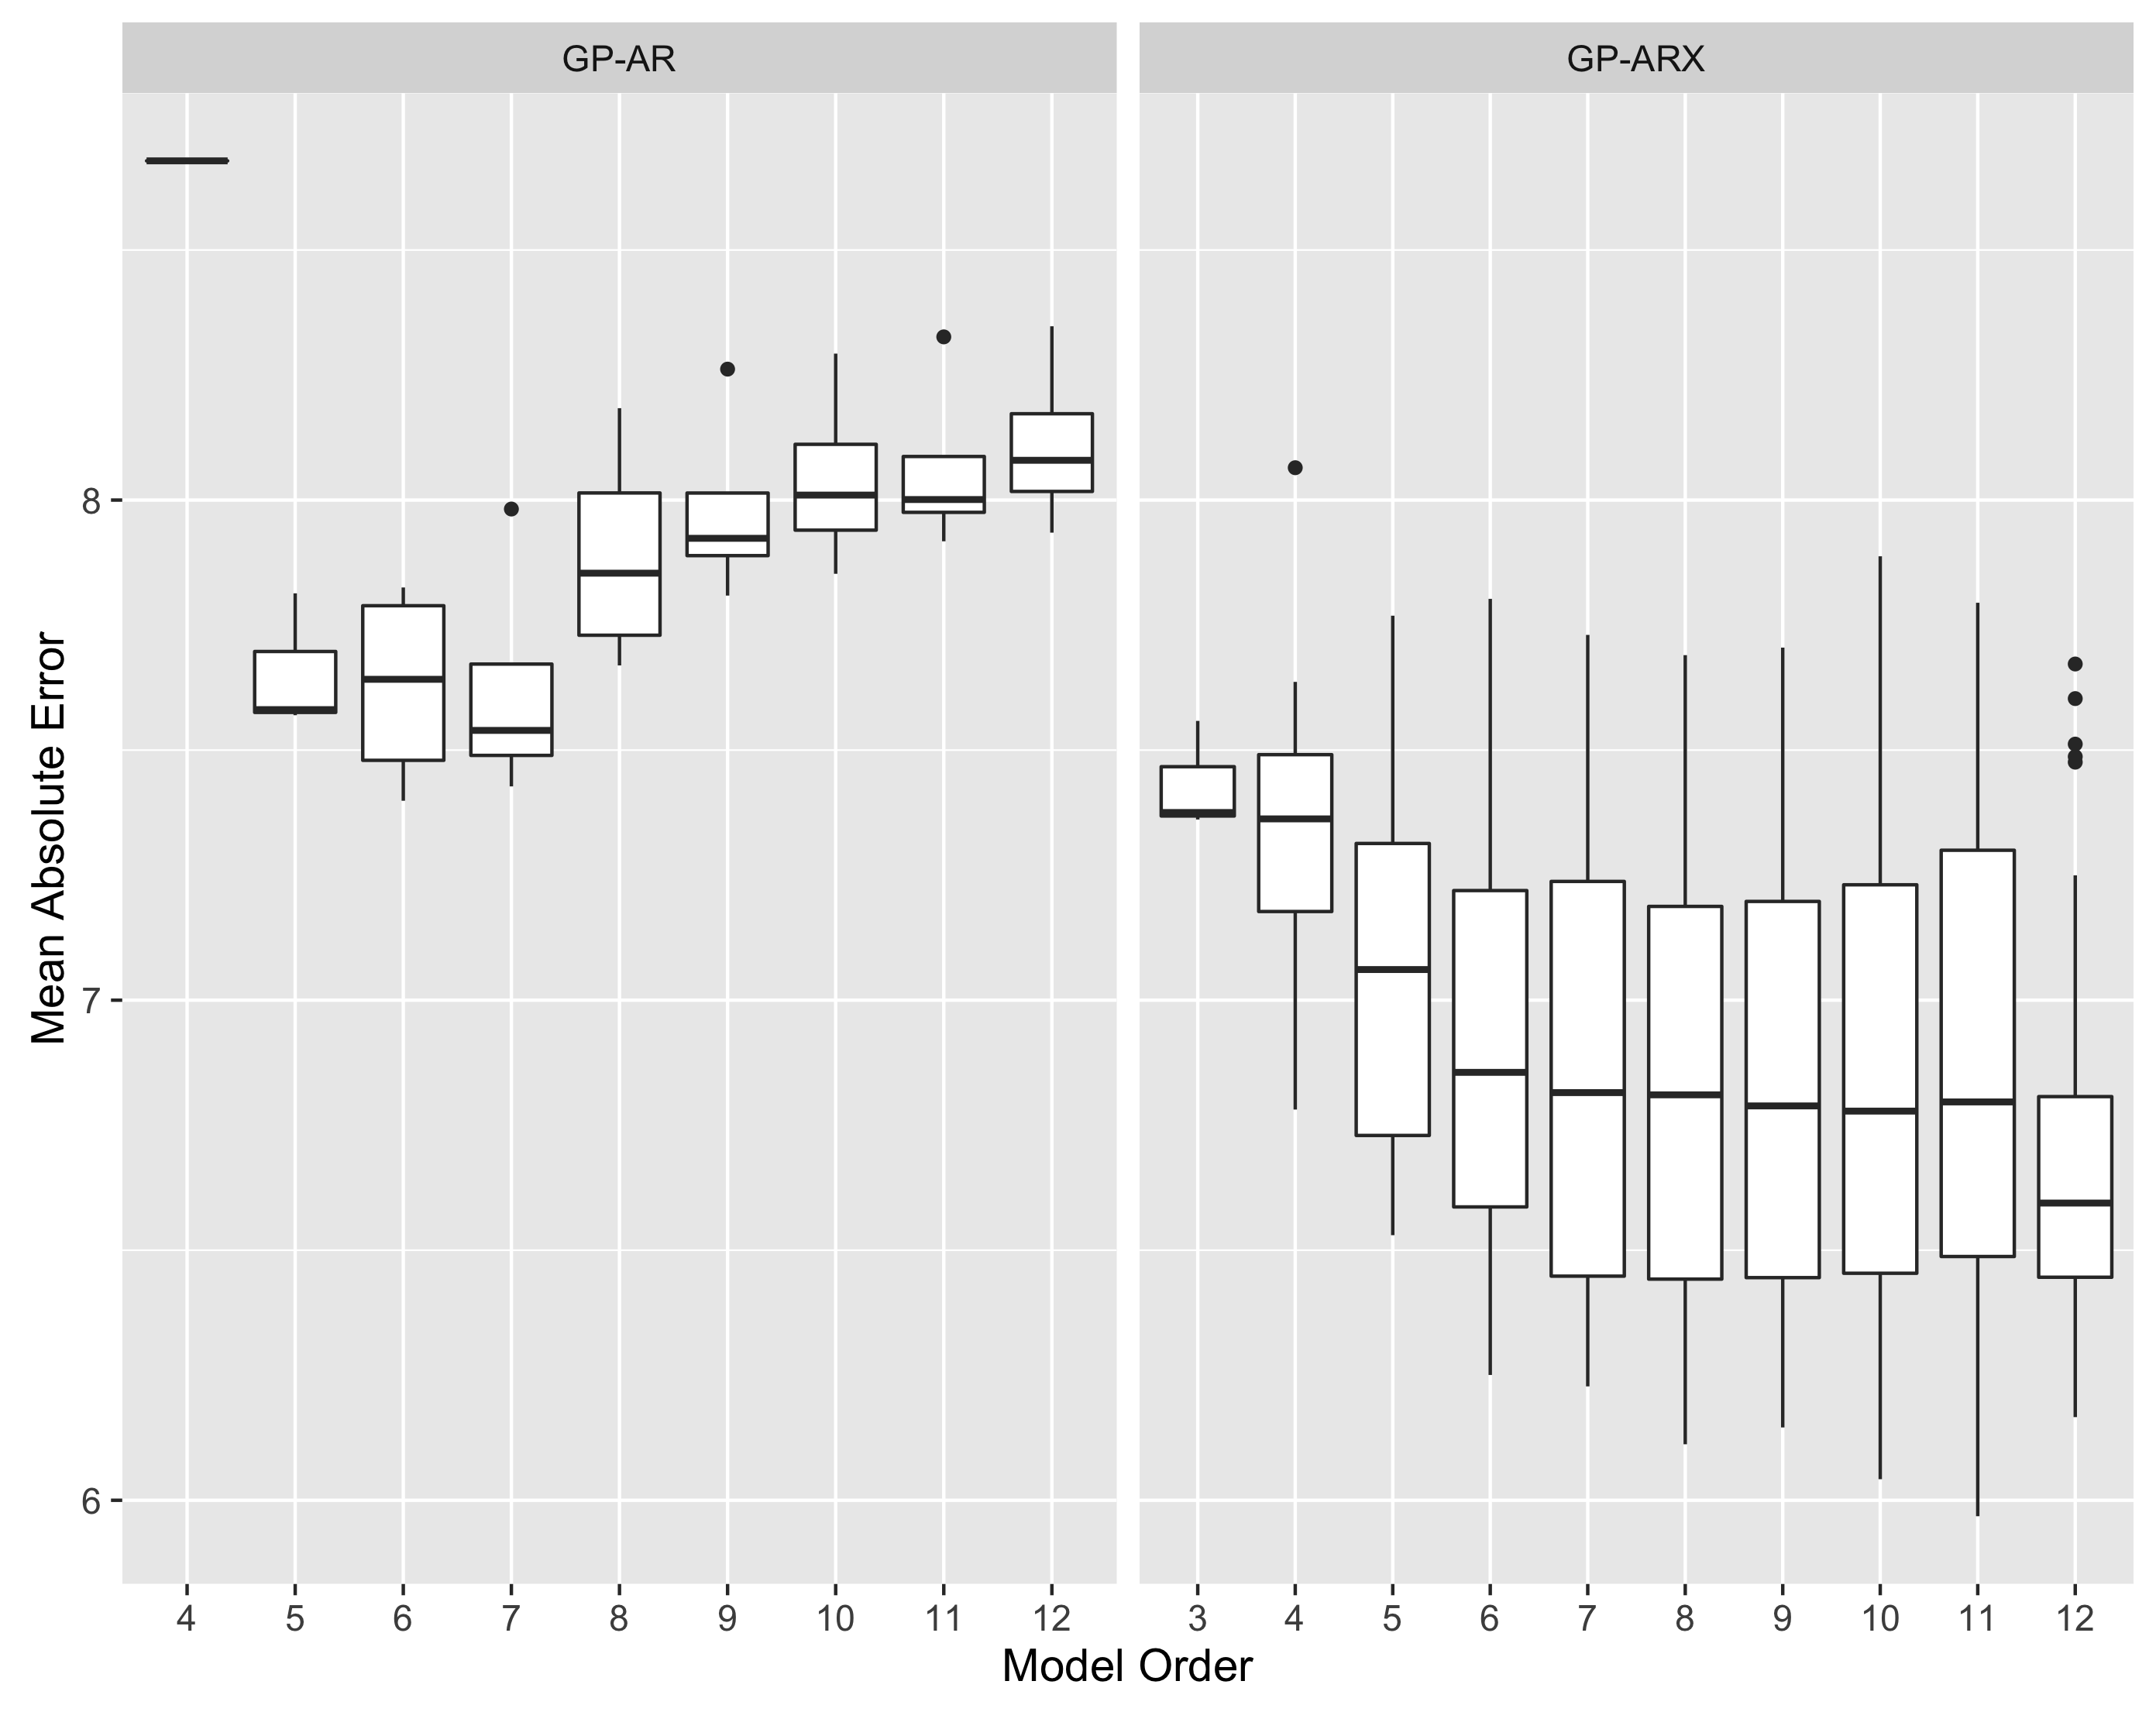
\includegraphics[width=\textwidth]{Compare-mae.png}
    \caption{Mean Absolute Error (\si{\nano\tesla}) on validation set storms vs model order for GP-AR and GP-ARX. \\ \textbf{Key}: Rectangle borders represent the first and third quartiles, with a horizontal line inside to indicate the median value, outlying points are shown as dots and whiskers indicate the smallest and largest non-outliers}
    \label{fig:CompareMae}
\end{figure}
    
\begin{figure}
    \noindent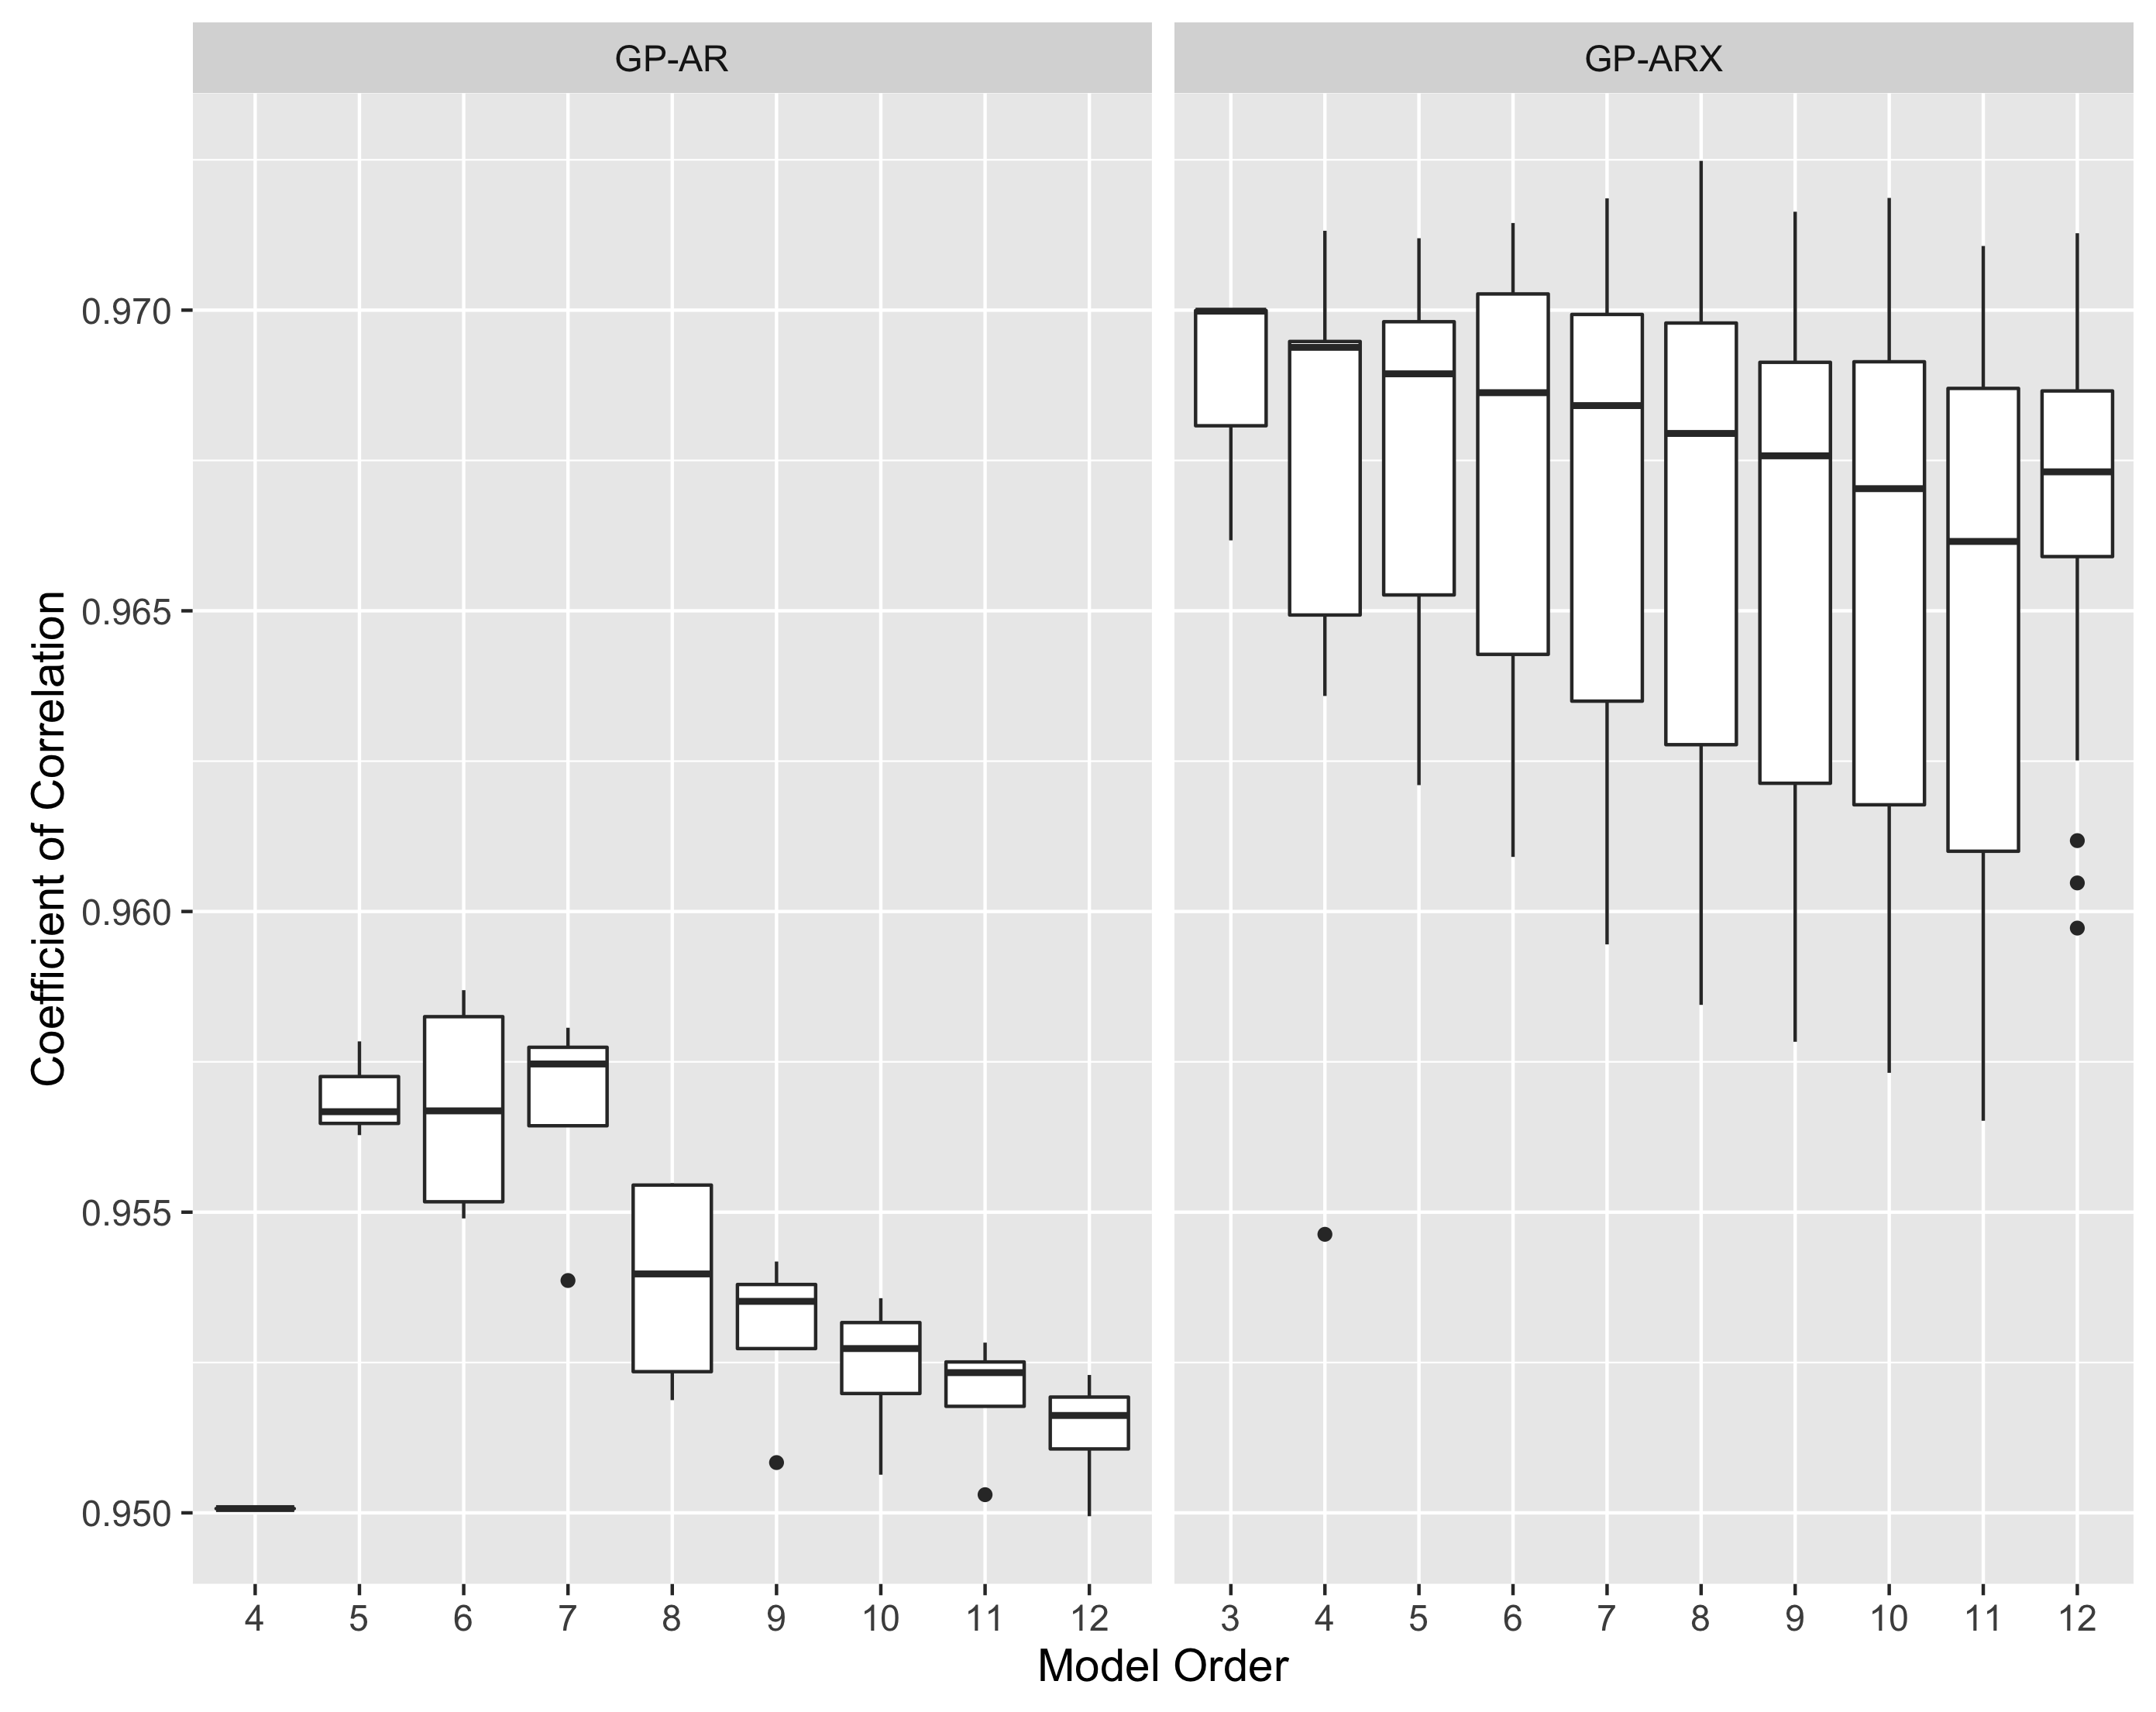
\includegraphics[width=\textwidth]{Compare-cc.png}
    \caption{Coefficient of Correlation on validation set storms vs model order for GP-AR and GP-ARX \\ \textbf{Key}: Rectangle borders represent the first and third quartiles, with a horizontal line inside to indicate the median value, outlying points are shown as dots and whiskers indicate the smallest and largest non-outliers}
    \label{fig:CompareCC}
\end{figure}
    
    
\begin{figure}
    \noindent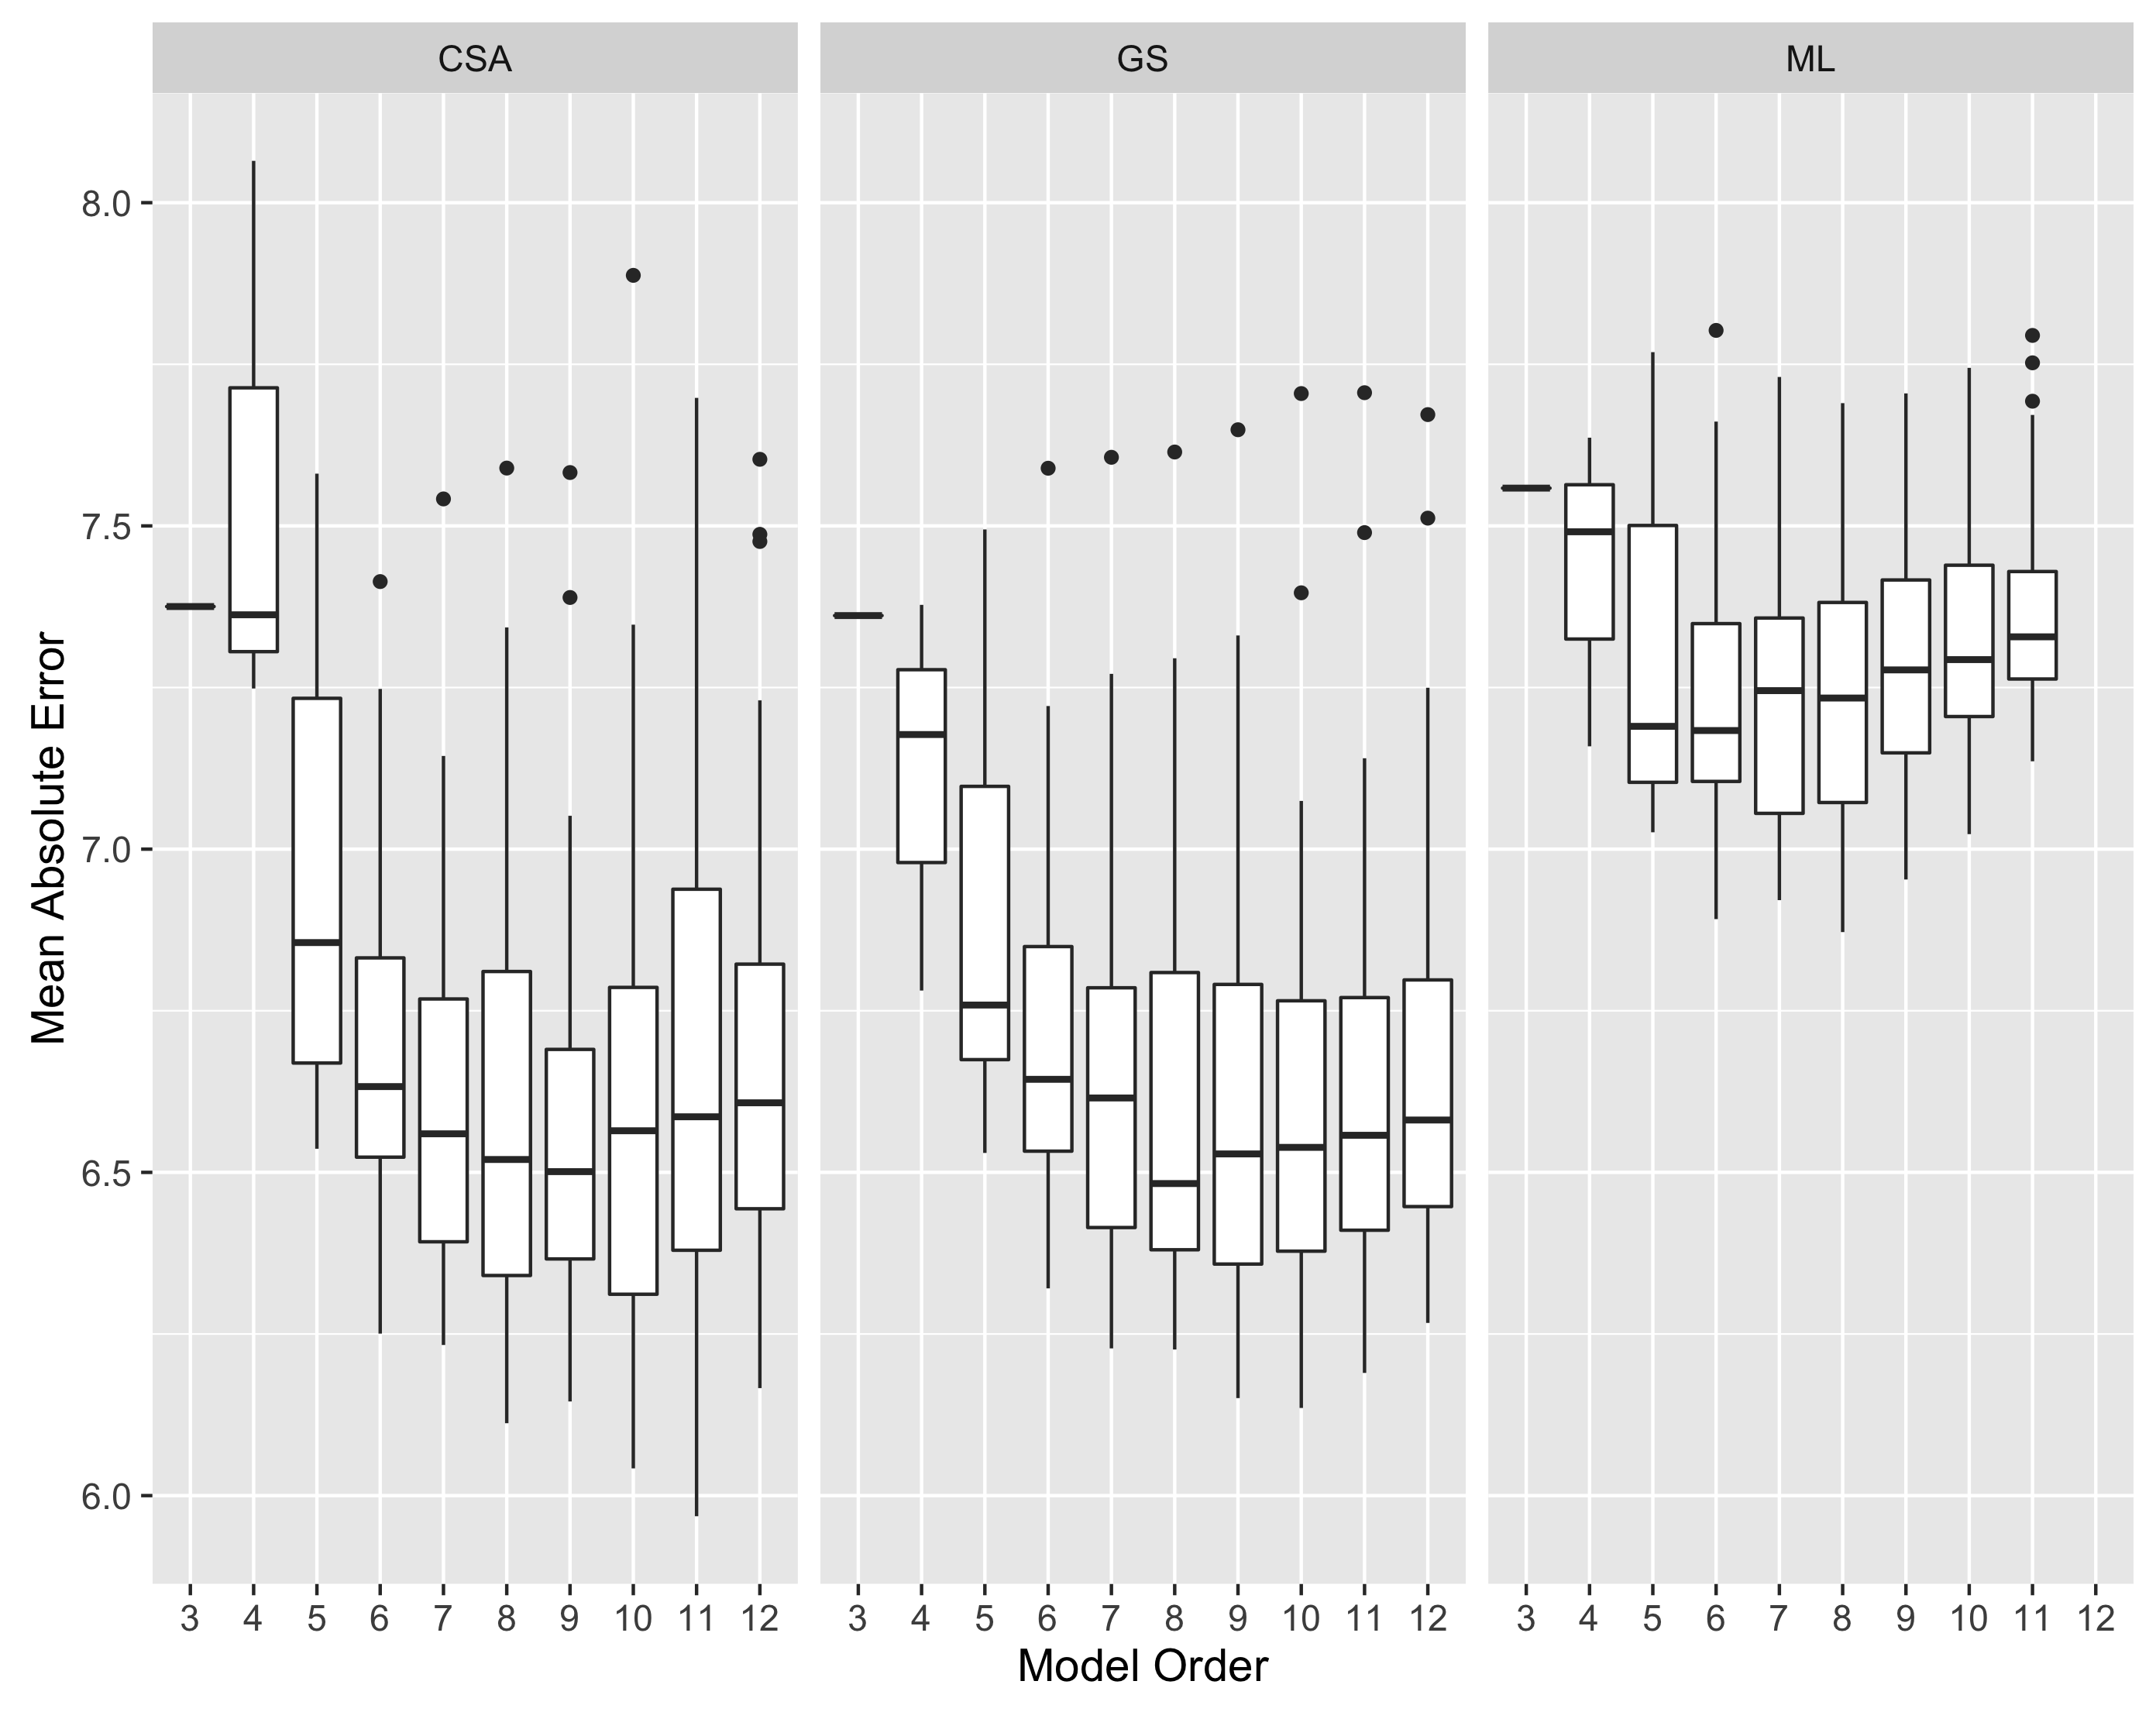
\includegraphics[width=\textwidth]{Compare-mae-arx.png}
    \caption{Mean Absolute Error (\si{\nano\tesla}) on validation set storms vs model order for GP-AR and GP-ARX for \emph{CSA}, \emph{GS} and \emph{ML} model selection routines \\ \textbf{Key}: Rectangle borders represent the first and third quartiles, with a horizontal line inside to indicate the median value, outlying points are shown as dots and whiskers indicate the smallest and largest non-outliers}
    \label{fig:CompareMaeARX}
\end{figure}
    
\begin{figure}
    \noindent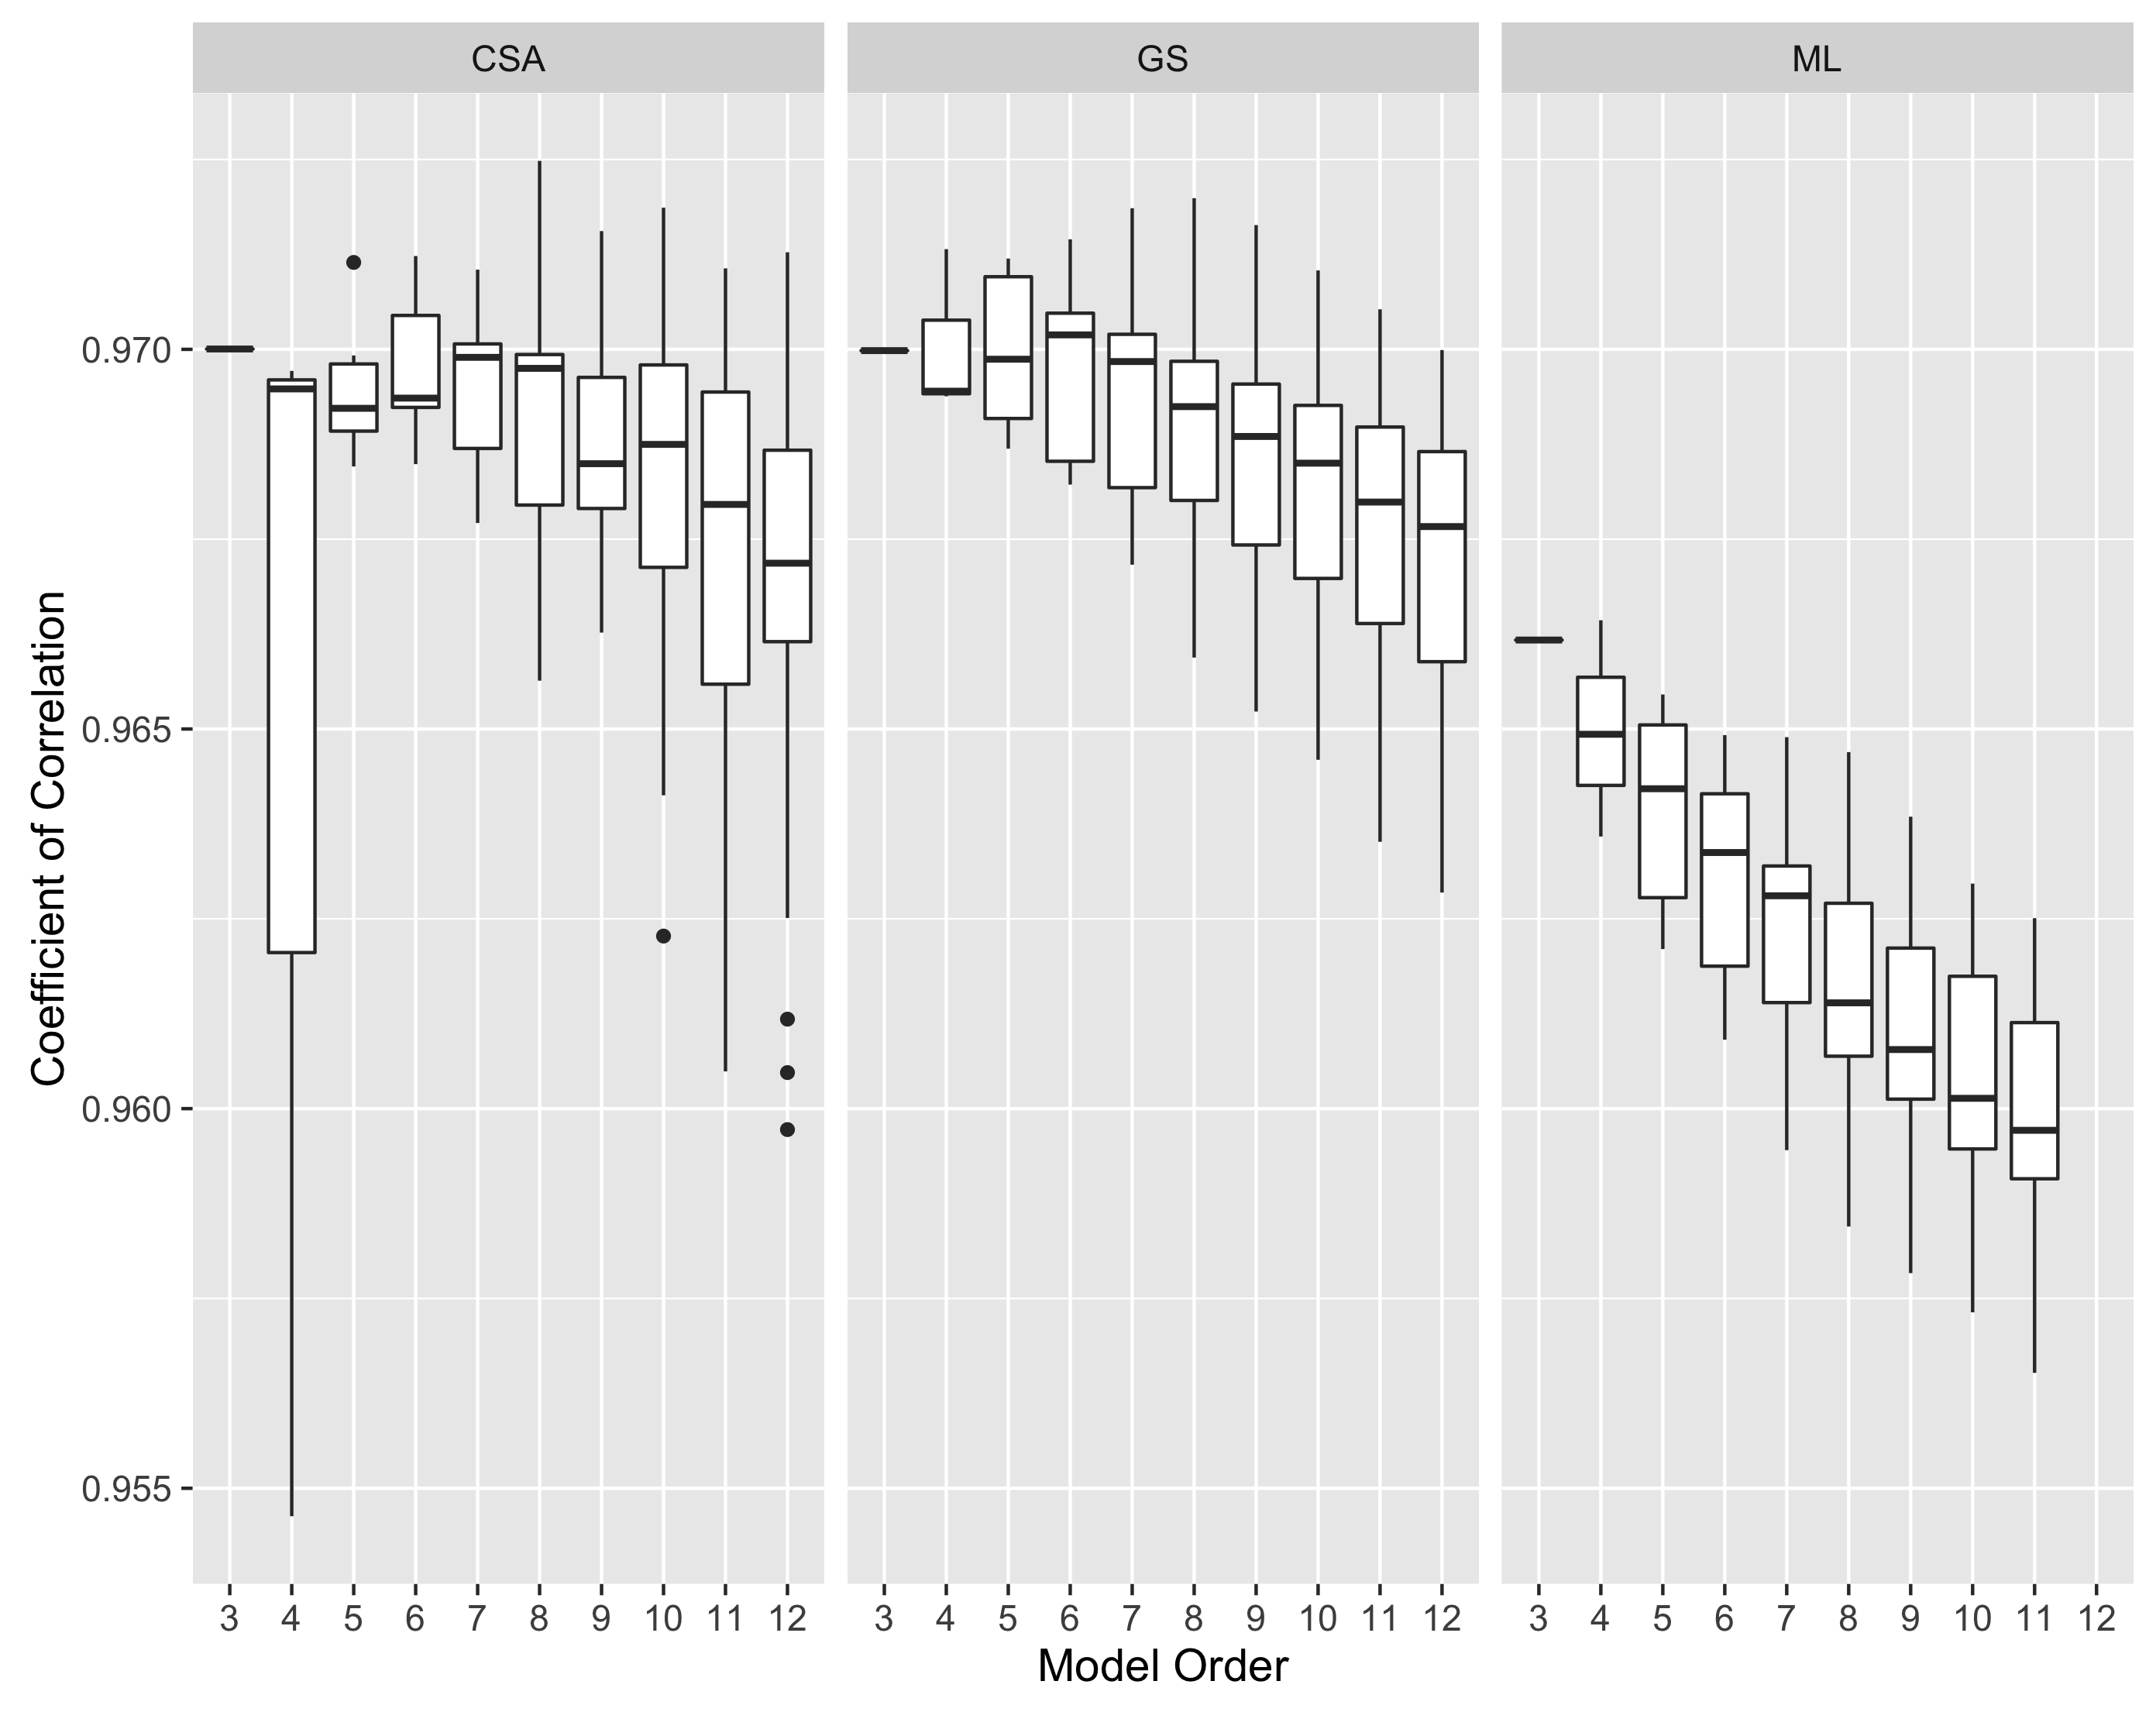
\includegraphics[width=\textwidth]{Compare-cc-arx.png}
    \caption{Coefficient of Correlation on validation set storms vs model order for GP-AR and GP-ARX for \emph{CSA}, \emph{GS} and \emph{ML} model selection routines \\ \textbf{Key}: Rectangle borders represent the first and third quartiles, with a horizontal line inside to indicate the median value, outlying points are shown as dots and whiskers indicate the smallest and largest non-outliers}
    \label{fig:CompareCCARX}
\end{figure}
    

\Cref{fig:CompareMae,fig:CompareCC} show how the mean absolute error and coefficient of correlation calculated on the validation set storm events from \cref{table:validationstorms}, vary with increasing model order for GP-AR and GP-ARX. The results are represented as box and whisker plots, in which a rectangle is drawn to represent the first and third quartiles, with a horizontal line inside to indicate the median value, outlying points are shown as dots while the whiskers indicate the smallest and largest non-outliers. In both cases, the predictive performance first improves and then stagnates or worsens with increasing model order. 

\Cref{fig:CompareMaeARX,fig:CompareCCARX} break down the results for GP-ARX by the model selection routine used. Apart from the general trend observed in \cref{fig:CompareMae,fig:CompareCC}, we also observe that \emph{grid search} and \emph{coupled simulated annealing} give superior performance as compared to gradient based \emph{maximum likelihood}.

From the validation results, we choose the model order which yields the best RMSE performance, for GP-AR it is $p_t = 6$ while for GP-ARX it is $p = 6, p_v = 1, p_b = 3$.

After choosing the best performing GP-AR and GP-ARX models, we calculate their performance on the test set of \cref{table:teststorms}. The results of these model evaluations are summarised in \cref{table:results}, the GP-AR and GP-ARX models improve upon the performance of the \emph{persistence model}.

\Cref{fig:ComparePred1,fig:ComparePred2,fig:ComparePred3} show OSA predictions of the GP-ARX model with $\pm \sigma$ error bars for three storm events in the time period between 1998 and 2003. The GP-ARX model gives accurate predictions along with plausible error bars around its mean predictions.

\section{Conclusions}

In this paper, we describe a flexible and expressive methodology for generating probabilistic forecasts of the $ \mathrm{Dst}$ index. We proposed two \emph{Gaussian Process} auto-regressive models, \emph{GP-ARX} and \emph{GP-AR}, to generate hourly predictions and their associated error bars. We also describe how to carry out model selection and validation of GP-AR and GP-ARX models.


Our results can be summarised as follows.
\begin{enumerate}
      \item \emph{Persistence} model plays an important role in the model building and evaluation process in the context of \emph{one step ahead} prediction of the $ \mathrm{Dst}$ index. Although it is not a robust predictor for the onset of intense geomagnetic storms, the \emph{persistence model} performs well on classical error metrics such as \emph{root mean square error} and such. From the considerations above, it is quite evident that classical performance metrics are not adequate for model evaluation, nevertheless in space weather literature, metrics such as \emph{RMSE} are very commonly used to compare predictive performance of models. Although not the research focus of this study, we note that there exists a need for the formulation of more informative performance metrics for measurement of predictive performance of geomagnetic predictive models.
      
      \item \emph{Gaussian Process} AR and ARX models give encouraging benefits in OSA prediction. Leveraging the strengths of the Bayesian approach, they are able to learn robust predictors from data. If one considers the size of the data used in our study, one can appreciate that the models presented here need relatively small training and validations sets: the training set contains 243 instances, while the validation set contains 782 instances.
      
      \item Since the GP models generate predictive distributions for test data and not just point predictions they lend themselves to the requirements of space weather prediction very well because of the need to generate error bars on predictions.
      
      \item The \emph{Gaussian Process} regression framework described in this study can also be extended to multiple hour ahead prediction of $ \mathrm{Dst}$, which is currently a work in progress.
\end{enumerate}




%%% End of body of article:

%%%%%%%%%%%%%%%%%%%%%%%%%%%%%%%%
%% Optional Appendix goes here
%
% \appendix resets counters and redefines section heads
% but doesn't print anything.
% After typing \appendix
%
%\section{Here Is Appendix Title}
% will show
% Appendix A: Here Is Appendix Title
%
%%%%%%%%%%%%%%%%%%%%%%%%%%%%%%%%%%%%%%%%%%%%%%%%%%%%%%%%%%%%%%%%
%
% Optional Glossary or Notation section, goes here
%

%%%%%%%%%%%%%%
% Notation -- End each entry with a period.
% \begin{notation}
% Term & definition.\\
% Second term & second definition.\\
% \end{notation}
%%%%%%%%%%%%%%%%%%%%%%%%%%%%%%%%%%%%%%%%%%%%%%%%%%%%%%%%%%%%%%%%
%
%  ACKNOWLEDGMENTS

%\begin{acknowledgments}
%We acknowledge use of NASA/GSFC's Space Physics Data Facility's OMNIWeb (or CDAWeb or ftp) service, and OMNI data. Simon Wing acknowledges supports from CWI and NSF Grant AGS-1058456 and NASA Grants (NNX13AE12G, NNX15AJ01G, NNX16AC39G).
%\end{acknowledgments}


    
\begin{figure}
    \noindent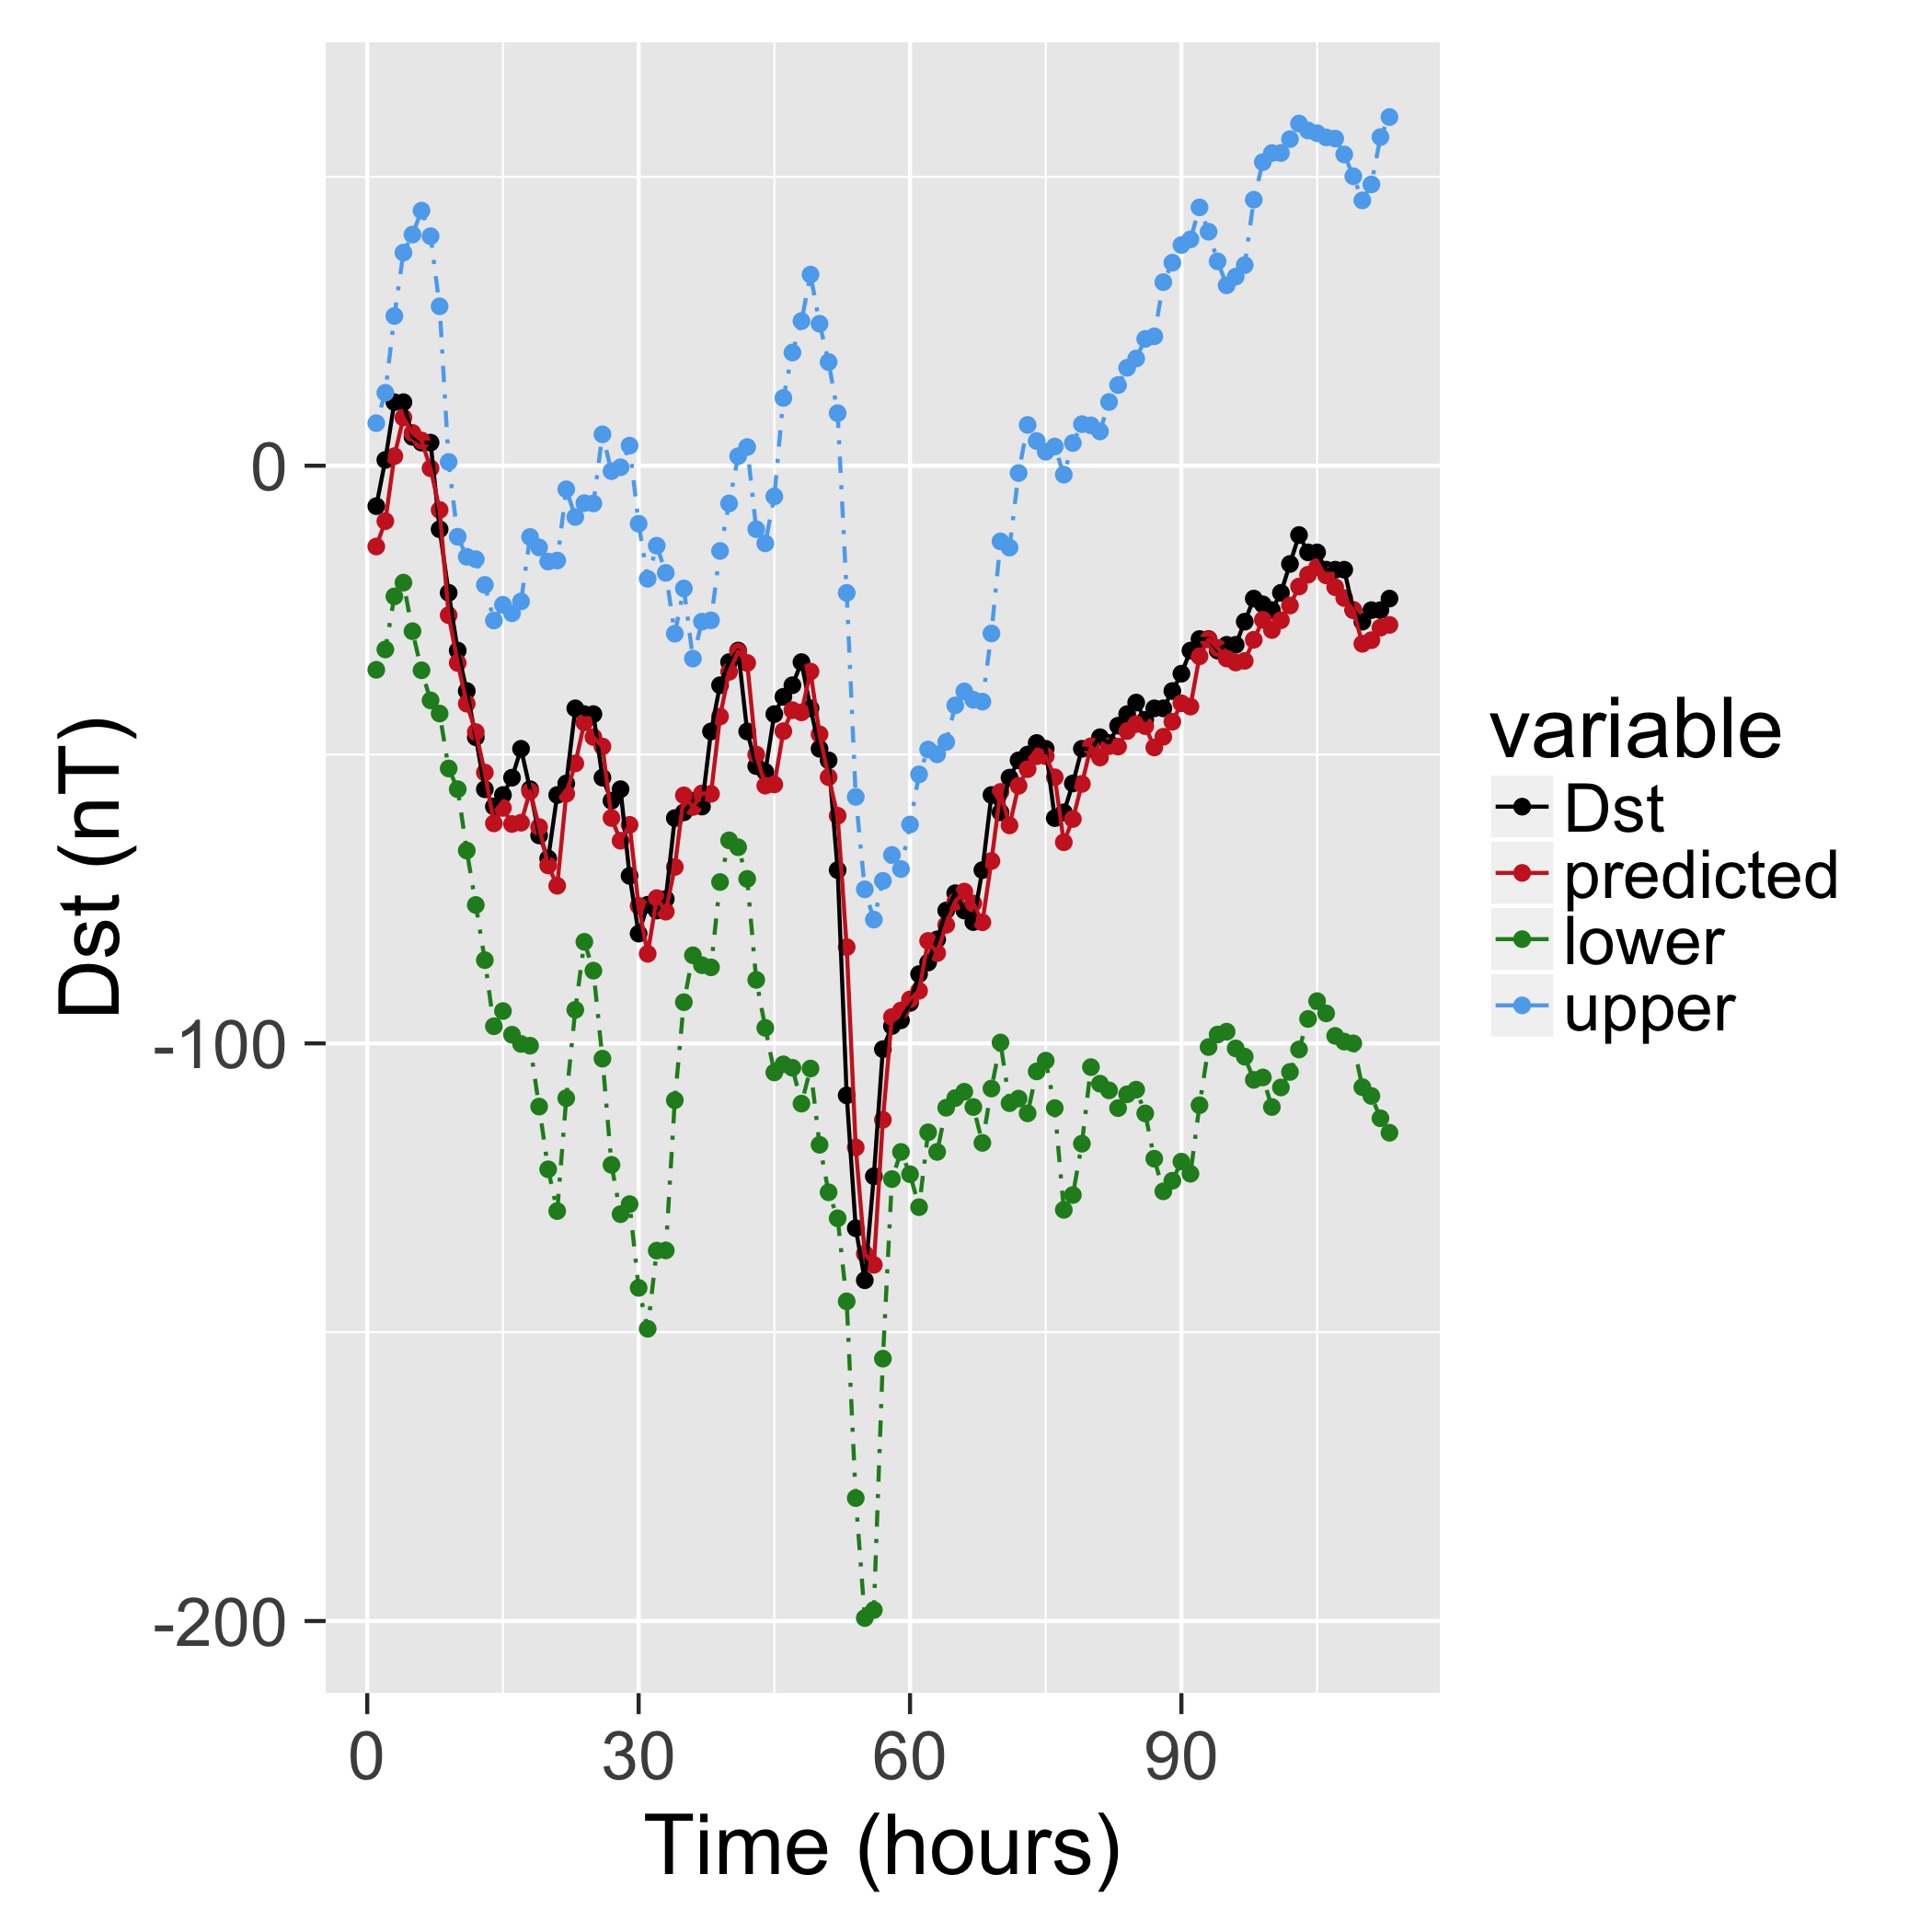
\includegraphics[width=\textwidth]{PredictionsModel1/PredErrBars_Storm43.png}
    \caption{OSA Predictions with $\pm \sigma$ error bars for event: 2003/06/17 to 2003/06/19}
    \label{fig:ComparePred1}
\end{figure}
    
    
\begin{figure}
    \noindent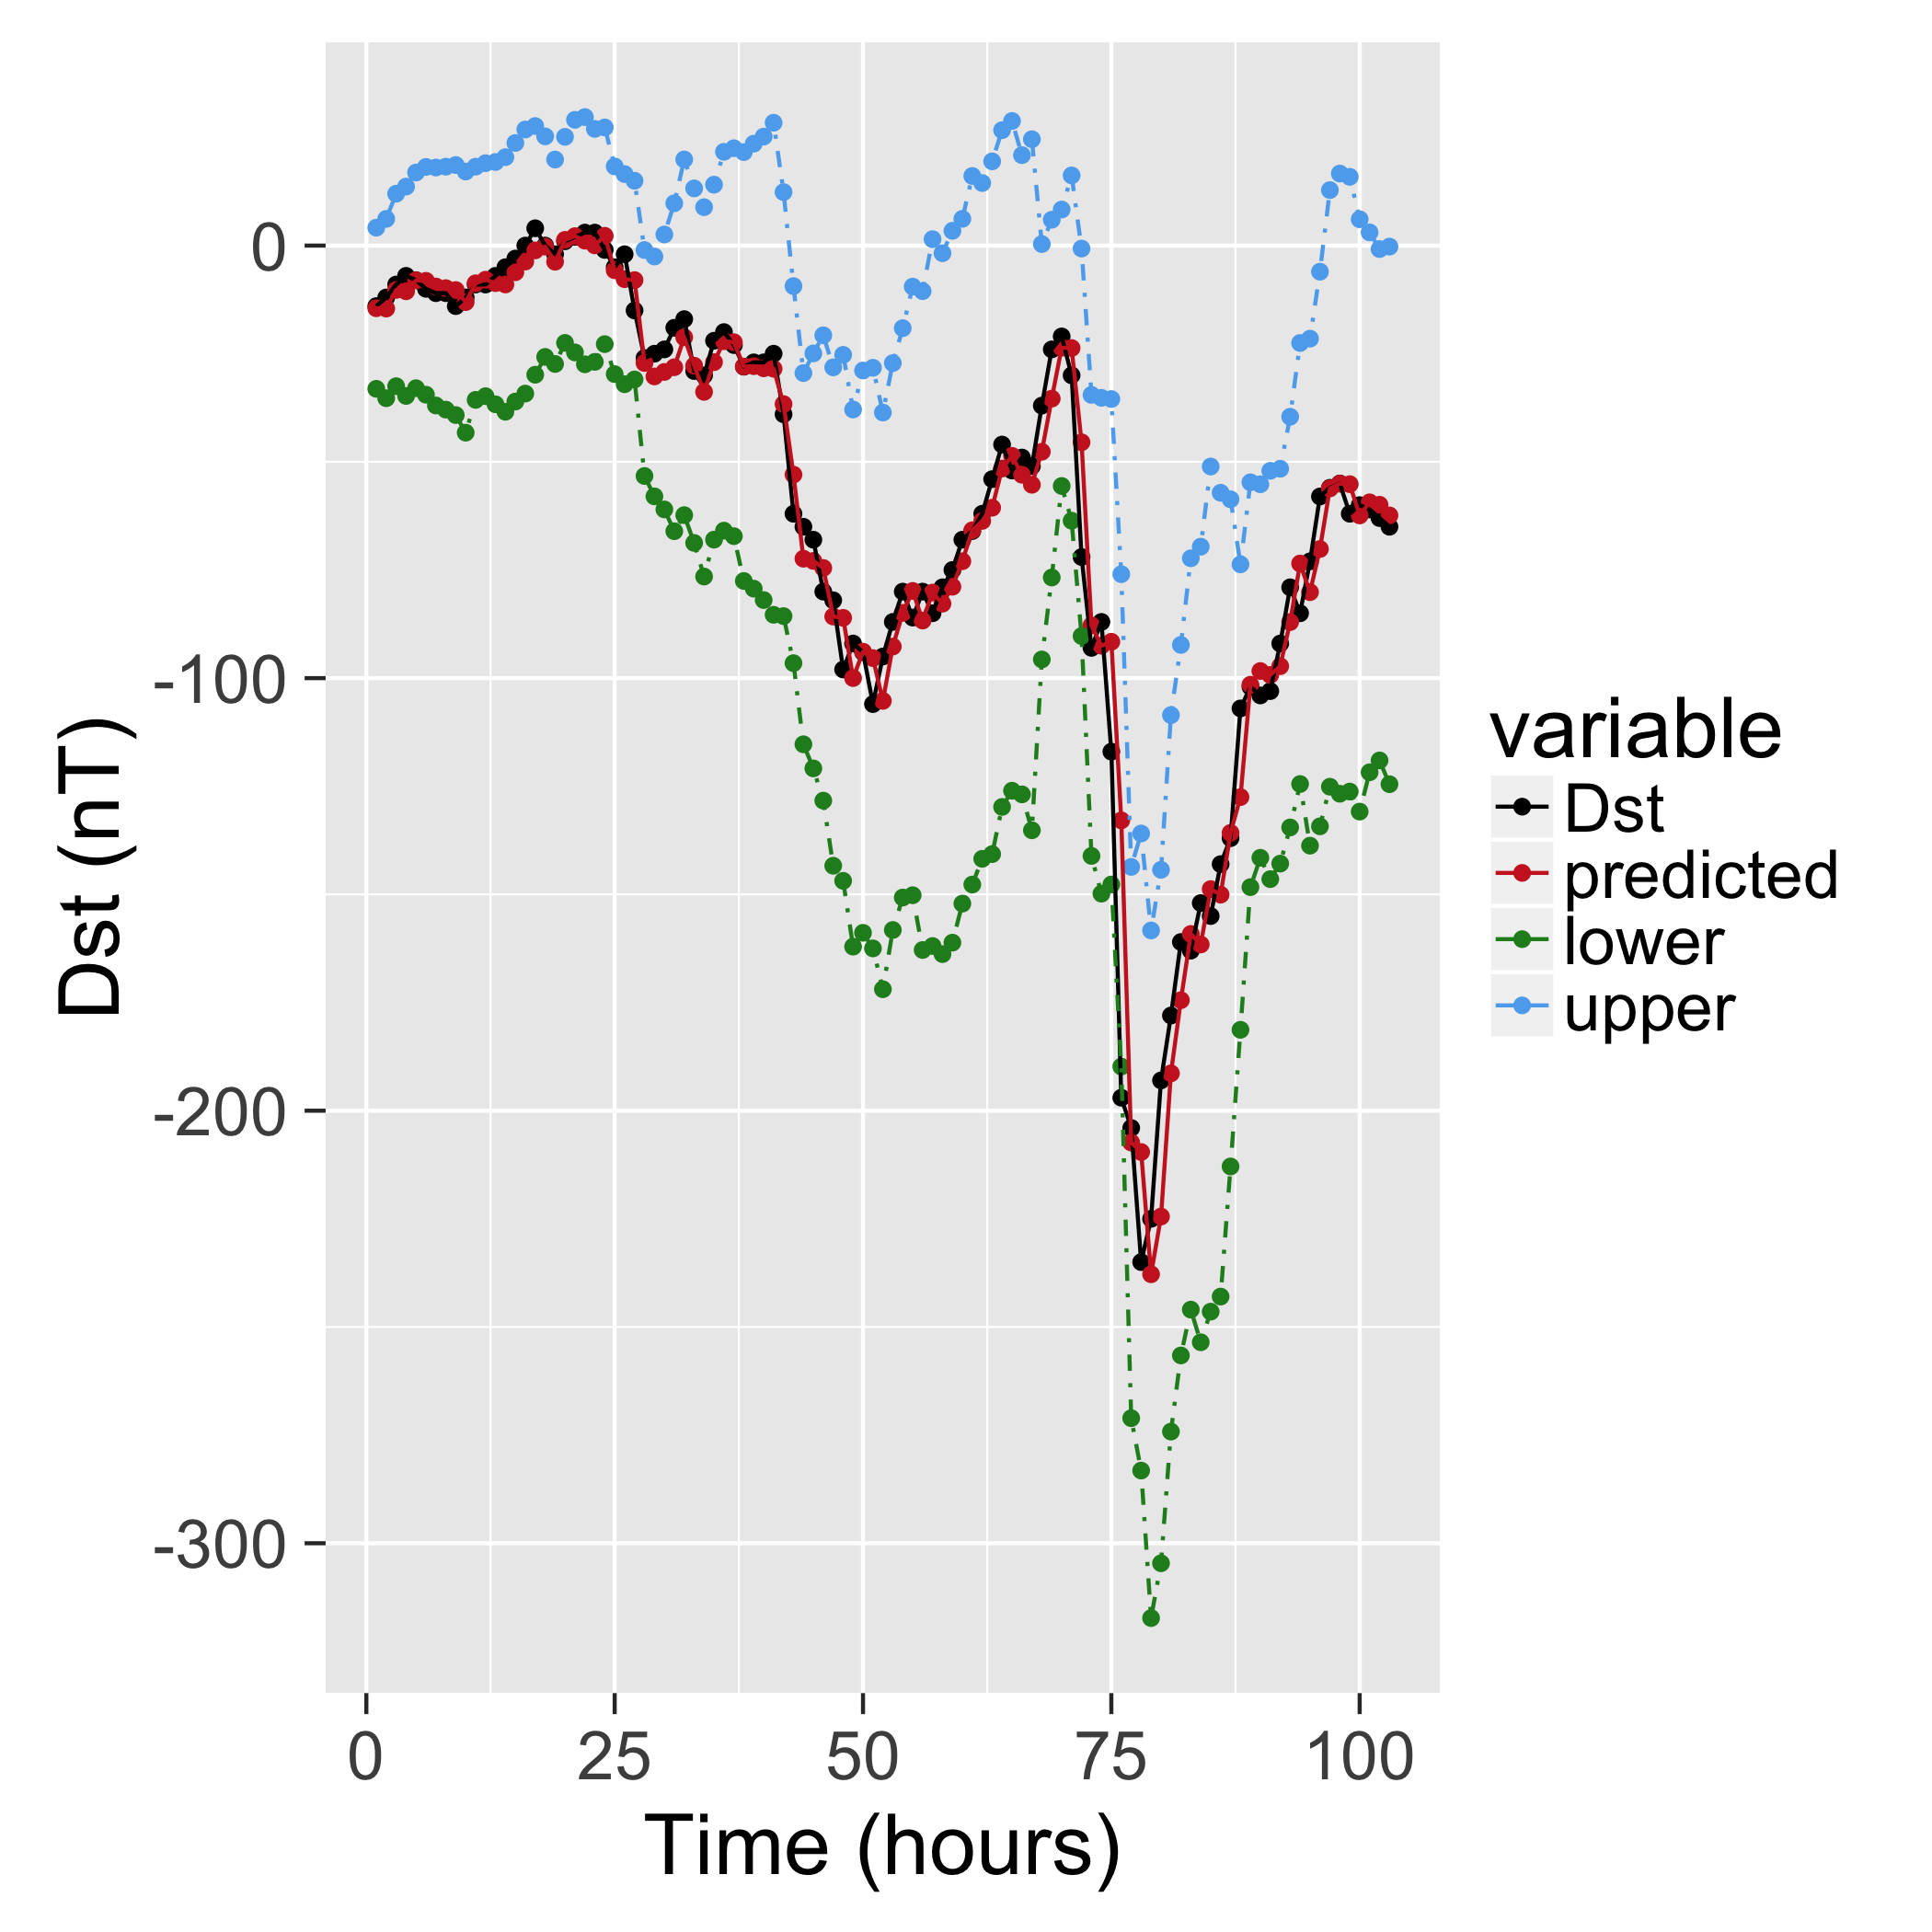
\includegraphics[width=\textwidth]{PredictionsModel1/PredErrBars_Storm16.png}
    \caption{OSA Predictions with $\pm \sigma$ error bars for event: 2012/03/08 to 2012/03/10}
    \label{fig:ComparePred2}
\end{figure}
    
\begin{figure}
    \noindent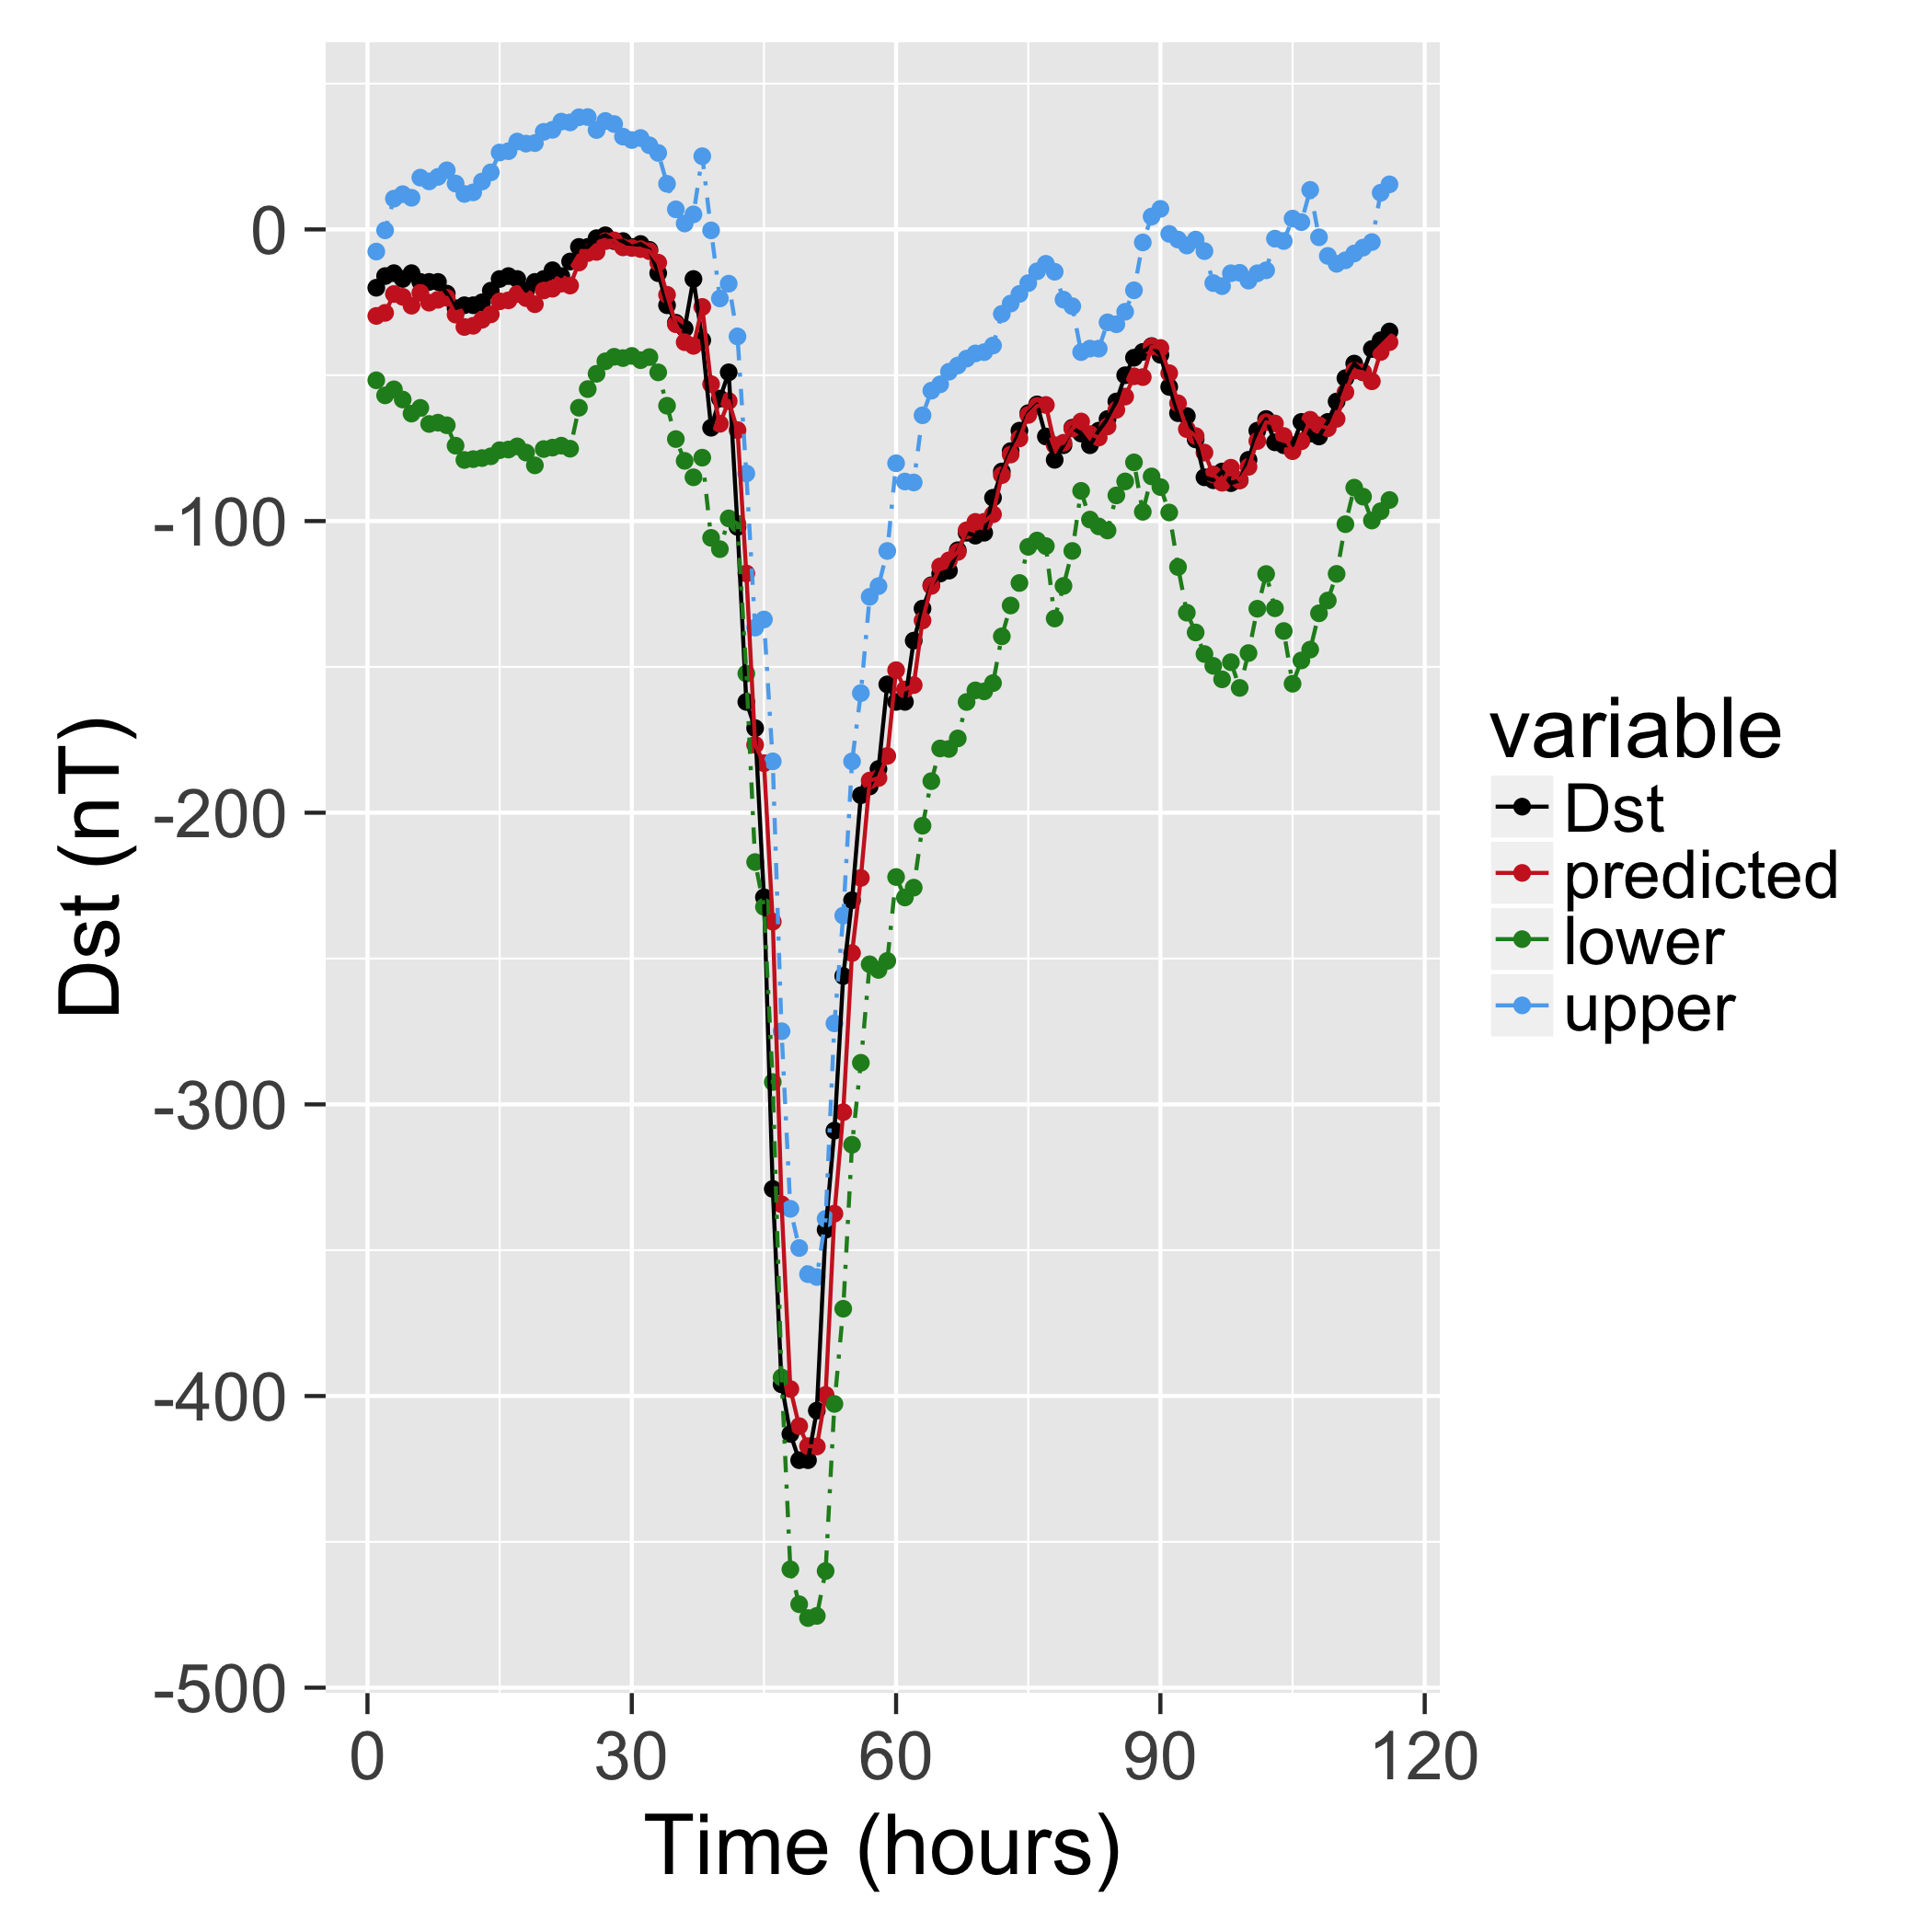
\includegraphics[width=\textwidth]{PredictionsModel1/PredErrBars_Storm46.png}
    \caption{OSA Predictions with $\pm \sigma$ error bars for event: 2003/11/20 to 2003/11/22}
    \label{fig:ComparePred3}
\end{figure}
    
    
    
    
    
    
\begin{table}[ht]
    \centering
    \caption{Storm events used for model selection of GP-AR and GP-ARX}
    \label{table:validationstorms}
    \begin{tabular}{llllll}
    \hline
    \textbf{Event Id} & \textbf{Start Date} & \textbf{Start Hour} & \textbf{End Date} & \textbf{End Hour} & \textbf{Storm Peak} \\ \hline
    1 & 1995/03/26 & 05:00 & 1995/03/26 & 23:00 & $ \SI{-107}{\nano\tesla}$ \\
    2 & 1995/04/07 & 13:00 & 1995/04/09 & 09:00 & $ \SI{-149}{\nano\tesla}$ \\
    3 & 1995/09/27 & 01:00 & 1995/09/28 & 04:00 & $ \SI{-108}{\nano\tesla}$ \\
    4 & 1995/10/18 & 13:00 & 1995/10/19 & 14:00 & $ \SI{-127}{\nano\tesla}$ \\
    5 & 1996/10/22 & 22:00 & 1996/10/23 & 11:00 & $ \SI{-105}{\nano\tesla}$ \\
    6 & 1997/04/21 & 10:00 & 1997/04/22 & 09:00 & $ \SI{-107}{\nano\tesla}$ \\
    7 & 1997/05/15 & 03:00 & 1997/05/16 & 00:00 & $ \SI{-115}{\nano\tesla}$ \\
    8 & 1997/10/10 & 18:00 & 1997/10/11 & 19:00 & $ \SI{-130}{\nano\tesla}$ \\
    9 & 1997/11/07 & 00:00 & 1997/11/07 & 18:00 & $ \SI{-110}{\nano\tesla}$ \\
    10 & 1997/11/22 & 21:00 & 1997/11/24 & 04:00 & $ \SI{-108}{\nano\tesla}$ \\
    11 & 2005/06/12 & 17:00 & 2005/06/13 & 19:00 & $ \SI{-106}{\nano\tesla}$ \\
    12 & 2005/08/31 & 12:00 & 2005/09/01 & 12:00 & $ \SI{-122}{\nano\tesla}$ \\
    13 & 2006/12/14 & 21:00 & 2006/12/16 & 03:00 & $ \SI{-162}{\nano\tesla}$ \\
    14 & 2011/09/26 & 14:00 & 2011/09/27 & 12:00 & $ \SI{-101}{\nano\tesla}$ \\
    15 & 2011/10/24 & 20:00 & 2011/10/25 & 14:00 & $ \SI{-132}{\nano\tesla}$ \\
    16 & 2012/03/08 & 12:00 & 2012/03/10 & 16:00 & $ \SI{-131}{\nano\tesla}$ \\
    17 & 2012/04/23 & 11:00 & 2012/04/24 & 13:00 & $ \SI{-108}{\nano\tesla}$ \\
    18 & 2012/07/15 & 01:00 & 2012/07/16 & 23:00 & $ \SI{-127}{\nano\tesla}$ \\
    19 & 2012/09/30 & 13:00 & 2012/10/01 & 18:00 & $ \SI{-119}{\nano\tesla}$ \\
    20 & 2012/10/08 & 02:00 & 2012/10/09 & 17:00 & $ \SI{-105}{\nano\tesla}$ \\
    21 & 2012/11/13 & 18:00 & 2012/11/14 & 18:00 & $ \SI{-108}{\nano\tesla}$ \\
    22 & 2013/03/17 & 07:00 & 2013/03/18 & 10:00 & $ \SI{-132}{\nano\tesla}$ \\
    23 & 2013/05/31 & 18:00 & 2013/06/01 & 20:00 & $ \SI{-119}{\nano\tesla}$ \\
    24 & 2014/02/18 & 15:00 & 2014/02/19 & 16:00 & $ \SI{-112}{\nano\tesla}$ \\ \hline
    \end{tabular}
    \end{table}
    
    

    \begin{table}[ht]
    %\fontsize{8}{9.6}\selectfont
    \centering
    \caption{Storm events used to evaluate GP-AR and GP-ARX models}
    \label{table:teststorms}
    \begin{adjustbox}{width=\textwidth,totalheight=0.9\textheight,keepaspectratio}
    \begin{tabular}{cccccc}
    \hline
    \textbf{Event Id} & \textbf{Start Date} & \textbf{Start Hour} & \textbf{End Date} & \textbf{End Hour} & \textbf{Storm Peak} \\ \hline
    1 & 1998/02/17 & 12:00 & 1998/02/18 & 10:00 & $ \SI{-100}{\nano\tesla}$ \\
    2 & 1998/03/10 & 11:00 & 1998/03/11 & 18:00 & $ \SI{-116}{\nano\tesla}$ \\
    3 & 1998/05/04 & 02:00 & 1998/05/05 & 02:00 & $ \SI{-205}{\nano\tesla}$ \\
    4 & 1998/08/26 & 10:00 & 1998/08/29 & 07:00 & $ \SI{-155}{\nano\tesla}$ \\
    5 & 1998/09/25 & 01:00 & 1998/09/26 & 00:00 & $ \SI{-207}{\nano\tesla}$ \\
    6 & 1998/10/19 & 05:00 & 1998/10/20 & 08:00 & $ \SI{-112}{\nano\tesla}$ \\
    7 & 1998/11/09 & 03:00 & 1998/11/10 & 16:00 & $ \SI{-142}{\nano\tesla}$ \\
    8 & 1998/11/13 & 00:00 & 1998/11/15 & 04:00 & $ \SI{-131}{\nano\tesla}$ \\
    9 & 1999/01/13 & 16:00 & 1999/01/14 & 20:00 & $ \SI{-112}{\nano\tesla}$ \\
    10 & 1999/02/18 & 03:00 & 1999/02/19 & 21:00 & $ \SI{-123}{\nano\tesla}$ \\
    11 & 1999/09/22 & 20:00 & 1999/09/23 & 23:00 & $ \SI{-173}{\nano\tesla}$ \\
    12 & 1999/10/22 & 00:00 & 1999/10/23 & 14:00 & $ \SI{-237}{\nano\tesla}$ \\
    13 & 2000/02/12 & 05:00 & 2000/02/13 & 15:00 & $ \SI{-133}{\nano\tesla}$ \\
    14 & 2000/04/06 & 17:00 & 2000/04/08 & 09:00 & $ \SI{-288}{\nano\tesla}$ \\
    15 & 2000/05/24 & 01:00 & 2000/05/25 & 20:00 & $ \SI{-147}{\nano\tesla}$ \\
    16 & 2000/08/10 & 20:00 & 2000/08/11 & 18:00 & $ \SI{-230}{\nano\tesla}$ \\
    17 & 2000/08/12 & 02:00 & 2000/08/13 & 17:00 & $ \SI{-235}{\nano\tesla}$ \\
    18 & 2000/10/13 & 02:00 & 2000/10/14 & 23:00 & $ \SI{-107}{\nano\tesla}$ \\
    19 & 2000/10/28 & 20:00 & 2000/10/29 & 20:00 & $ \SI{-127}{\nano\tesla}$ \\
    20 & 2000/11/06 & 13:00 & 2000/11/07 & 18:00 & $ \SI{-159}{\nano\tesla}$ \\
    21 & 2000/11/28 & 18:00 & 2000/11/29 & 23:00 & $ \SI{-119}{\nano\tesla}$ \\
    22 & 2001/03/19 & 15:00 & 2001/03/21 & 23:00 & $ \SI{-149}{\nano\tesla}$ \\
    23 & 2001/03/31 & 04:00 & 2001/04/01 & 21:00 & $ \SI{-387}{\nano\tesla}$ \\
    24 & 2001/04/11 & 16:00 & 2001/04/13 & 07:00 & $ \SI{-271}{\nano\tesla}$ \\
    25 & 2001/04/18 & 01:00 & 2001/04/18 & 13:00 & $ \SI{-114}{\nano\tesla}$ \\
    26 & 2001/04/22 & 02:00 & 2001/04/23 & 15:00 & $ \SI{-102}{\nano\tesla}$ \\
    27 & 2001/08/17 & 16:00 & 2001/08/18 & 16:00 & $ \SI{-105}{\nano\tesla}$ \\
    28 & 2001/09/30 & 23:00 & 2001/10/02 & 00:00 & $ \SI{-148}{\nano\tesla}$ \\
    29 & 2001/10/21 & 17:00 & 2001/10/24 & 11:00 & $ \SI{-187}{\nano\tesla}$ \\
    30 & 2001/10/28 & 03:00 & 2001/10/29 & 22:00 & $ \SI{-157}{\nano\tesla}$ \\
    31 & 2002/03/23 & 14:00 & 2002/03/25 & 05:00 & $ \SI{-100}{\nano\tesla}$ \\
    32 & 2002/04/17 & 11:00 & 2002/04/19 & 02:00 & $ \SI{-127}{\nano\tesla}$ \\
    33 & 2002/04/19 & 09:00 & 2002/04/21 & 06:00 & $ \SI{-149}{\nano\tesla}$ \\
    34 & 2002/05/11 & 10:00 & 2002/05/12 & 16:00 & $ \SI{-110}{\nano\tesla}$ \\
    35 & 2002/05/23 & 12:00 & 2002/05/24 & 23:00 & $ \SI{-109}{\nano\tesla}$ \\
    36 & 2002/08/01 & 23:00 & 2002/08/02 & 09:00 & $ \SI{-102}{\nano\tesla}$ \\
    37 & 2002/09/04 & 01:00 & 2002/09/05 & 00:00 & $ \SI{-109}{\nano\tesla}$ \\
    38 & 2002/09/07 & 14:00 & 2002/09/08 & 20:00 & $ \SI{-181}{\nano\tesla}$ \\
    39 & 2002/10/01 & 06:00 & 2002/10/03 & 08:00 & $ \SI{-176}{\nano\tesla}$ \\
    40 & 2002/10/03 & 10:00 & 2002/10/04 & 18:00 & $ \SI{-146}{\nano\tesla}$ \\
    41 & 2002/11/20 & 16:00 & 2002/11/22 & 06:00 & $ \SI{-128}{\nano\tesla}$ \\
    42 & 2003/05/29 & 20:00 & 2003/05/30 & 10:00 & $ \SI{-144}{\nano\tesla}$ \\
    43 & 2003/06/17 & 19:00 & 2003/06/19 & 03:00 & $ \SI{-141}{\nano\tesla}$ \\
    44 & 2003/07/11 & 15:00 & 2003/07/12 & 16:00 & $ \SI{-105}{\nano\tesla}$ \\
    45 & 2003/08/17 & 18:00 & 2003/08/19 & 11:00 & $ \SI{-148}{\nano\tesla}$ \\
    46 & 2003/11/20 & 12:00 & 2003/11/22 & 00:00 & $ \SI{-422}{\nano\tesla}$ \\
    47 & 2004/01/22 & 03:00 & 2004/01/24 & 00:00 & $ \SI{-149}{\nano\tesla}$ \\
    48 & 2004/02/11 & 10:00 & 2004/02/12 & 00:00 & $ \SI{-105}{\nano\tesla}$ \\
    49 & 2004/04/03 & 14:00 & 2004/04/04 & 08:00 & $ \SI{-112}{\nano\tesla}$ \\
    50 & 2004/07/22 & 20:00 & 2004/07/23 & 20:00 & $ \SI{-101}{\nano\tesla}$ \\
    51 & 2004/07/24 & 21:00 & 2004/07/26 & 17:00 & $ \SI{-148}{\nano\tesla}$ \\
    52 & 2004/07/26 & 22:00 & 2004/07/30 & 05:00 & $ \SI{-197}{\nano\tesla}$ \\
    53 & 2004/08/30 & 05:00 & 2004/08/31 & 21:00 & $ \SI{-126}{\nano\tesla}$ \\
    54 & 2004/11/07 & 21:00 & 2004/11/08 & 21:00 & $ \SI{-373}{\nano\tesla}$ \\
    55 & 2004/11/09 & 11:00 & 2004/11/11 & 09:00 & $ \SI{-289}{\nano\tesla}$ \\
    56 & 2004/11/11 & 22:00 & 2004/11/13 & 13:00 & $ \SI{-109}{\nano\tesla}$ \\
    57 & 2005/01/21 & 18:00 & 2005/01/23 & 05:00 & $ \SI{-105}{\nano\tesla}$ \\
    58 & 2005/05/07 & 20:00 & 2005/05/09 & 10:00 & $ \SI{-127}{\nano\tesla}$ \\
    59 & 2005/05/29 & 22:00 & 2005/05/31 & 08:00 & $ \SI{-138}{\nano\tesla}$ \\
    60 & 2005/06/12 & 17:00 & 2005/06/13 & 19:00 & $ \SI{-106}{\nano\tesla}$ \\
    61 & 2005/08/31 & 12:00 & 2005/09/01 & 12:00 & $ \SI{-131}{\nano\tesla}$ \\
    62 & 2006/04/13 & 20:00 & 2006/04/14 & 23:00 & $ \SI{-111}{\nano\tesla}$ \\
    63 & 2006/12/14 & 21:00 & 2006/12/16 & 03:00 & $ \SI{-147}{\nano\tesla}$ \\ \hline
    \end{tabular}%
    \end{adjustbox}
    \end{table}
    

%\bibliographystyle{plainnat}
%\bibliography{references}
